\section{Supplementary Material}

As supplementary material, we present and review a number of input/output examples across several categories with distinct properties\footnote{Link to audiovisual examples page: \href{https://web.media.mit.edu/~nsingh1/image2reverb/}{https://web.media.mit.edu/~nsingh1/image2reverb/}}. A summary of these results is shown in Table \ref{tab:results}. We additionally present a more detailed diagram of our architecture, shown in Fig. \ref{fig:nn_arch}.

Finally, to gain a qualitative view of intra-scene and adjacent-scene consistency, we plot our test set input images according to the corresponding output audio characteristics by a visualization shown in Figure \ref{fig:tsne}. We produce multiband $T_{60}$ estimations from all output IRs, and then used t-SNE \cite{maaten2008visualizing} to reduce the data dimensionality to two dimensions. We then solve a linear assignment problem to transform this into a grid representation. Several instances of within-scene clusters are visible, as well as closeness of related scenes. This suggests that while our method does make errors (outliers are also visible), it learns to treat similar scenes similarly while capturing variation.


\begin{table}[!h]
    \centering
    \begin{tabular}{l|c|c}
         \textbf{Topic} &  \textbf{Figure \#} & \textbf{Images}\\
         \hline
         Famous and iconic places & \ref{fig:p_famous} & 6\\
         Musical environments & \ref{fig:p_music} & 6\\
         Artistic renderings & \ref{fig:p_art} & 6\\
         DALL•E-generated spaces & \ref{fig:p_dall-e} & 6\\
         Limitations (i.e. challenging examples) & \ref{fig:p_reflection} & 4\\
         Animated scenes & \ref{fig:p_animation} & 6\\
         Virtual backgrounds & \ref{fig:p_zoom} & 6\\
         Historical places & \ref{fig:p_other} & 5\\
         Video games & \ref{fig:p_videogame} & 4\\
         Common and identifiable scenes & \ref{fig:p_everyday} & 6\\
         \hline
         Total & & 55\\
    \end{tabular}
    \caption{Additional Results.}
    \label{tab:results}
\end{table}

\begin{figure*}[!hb]
    \centering
    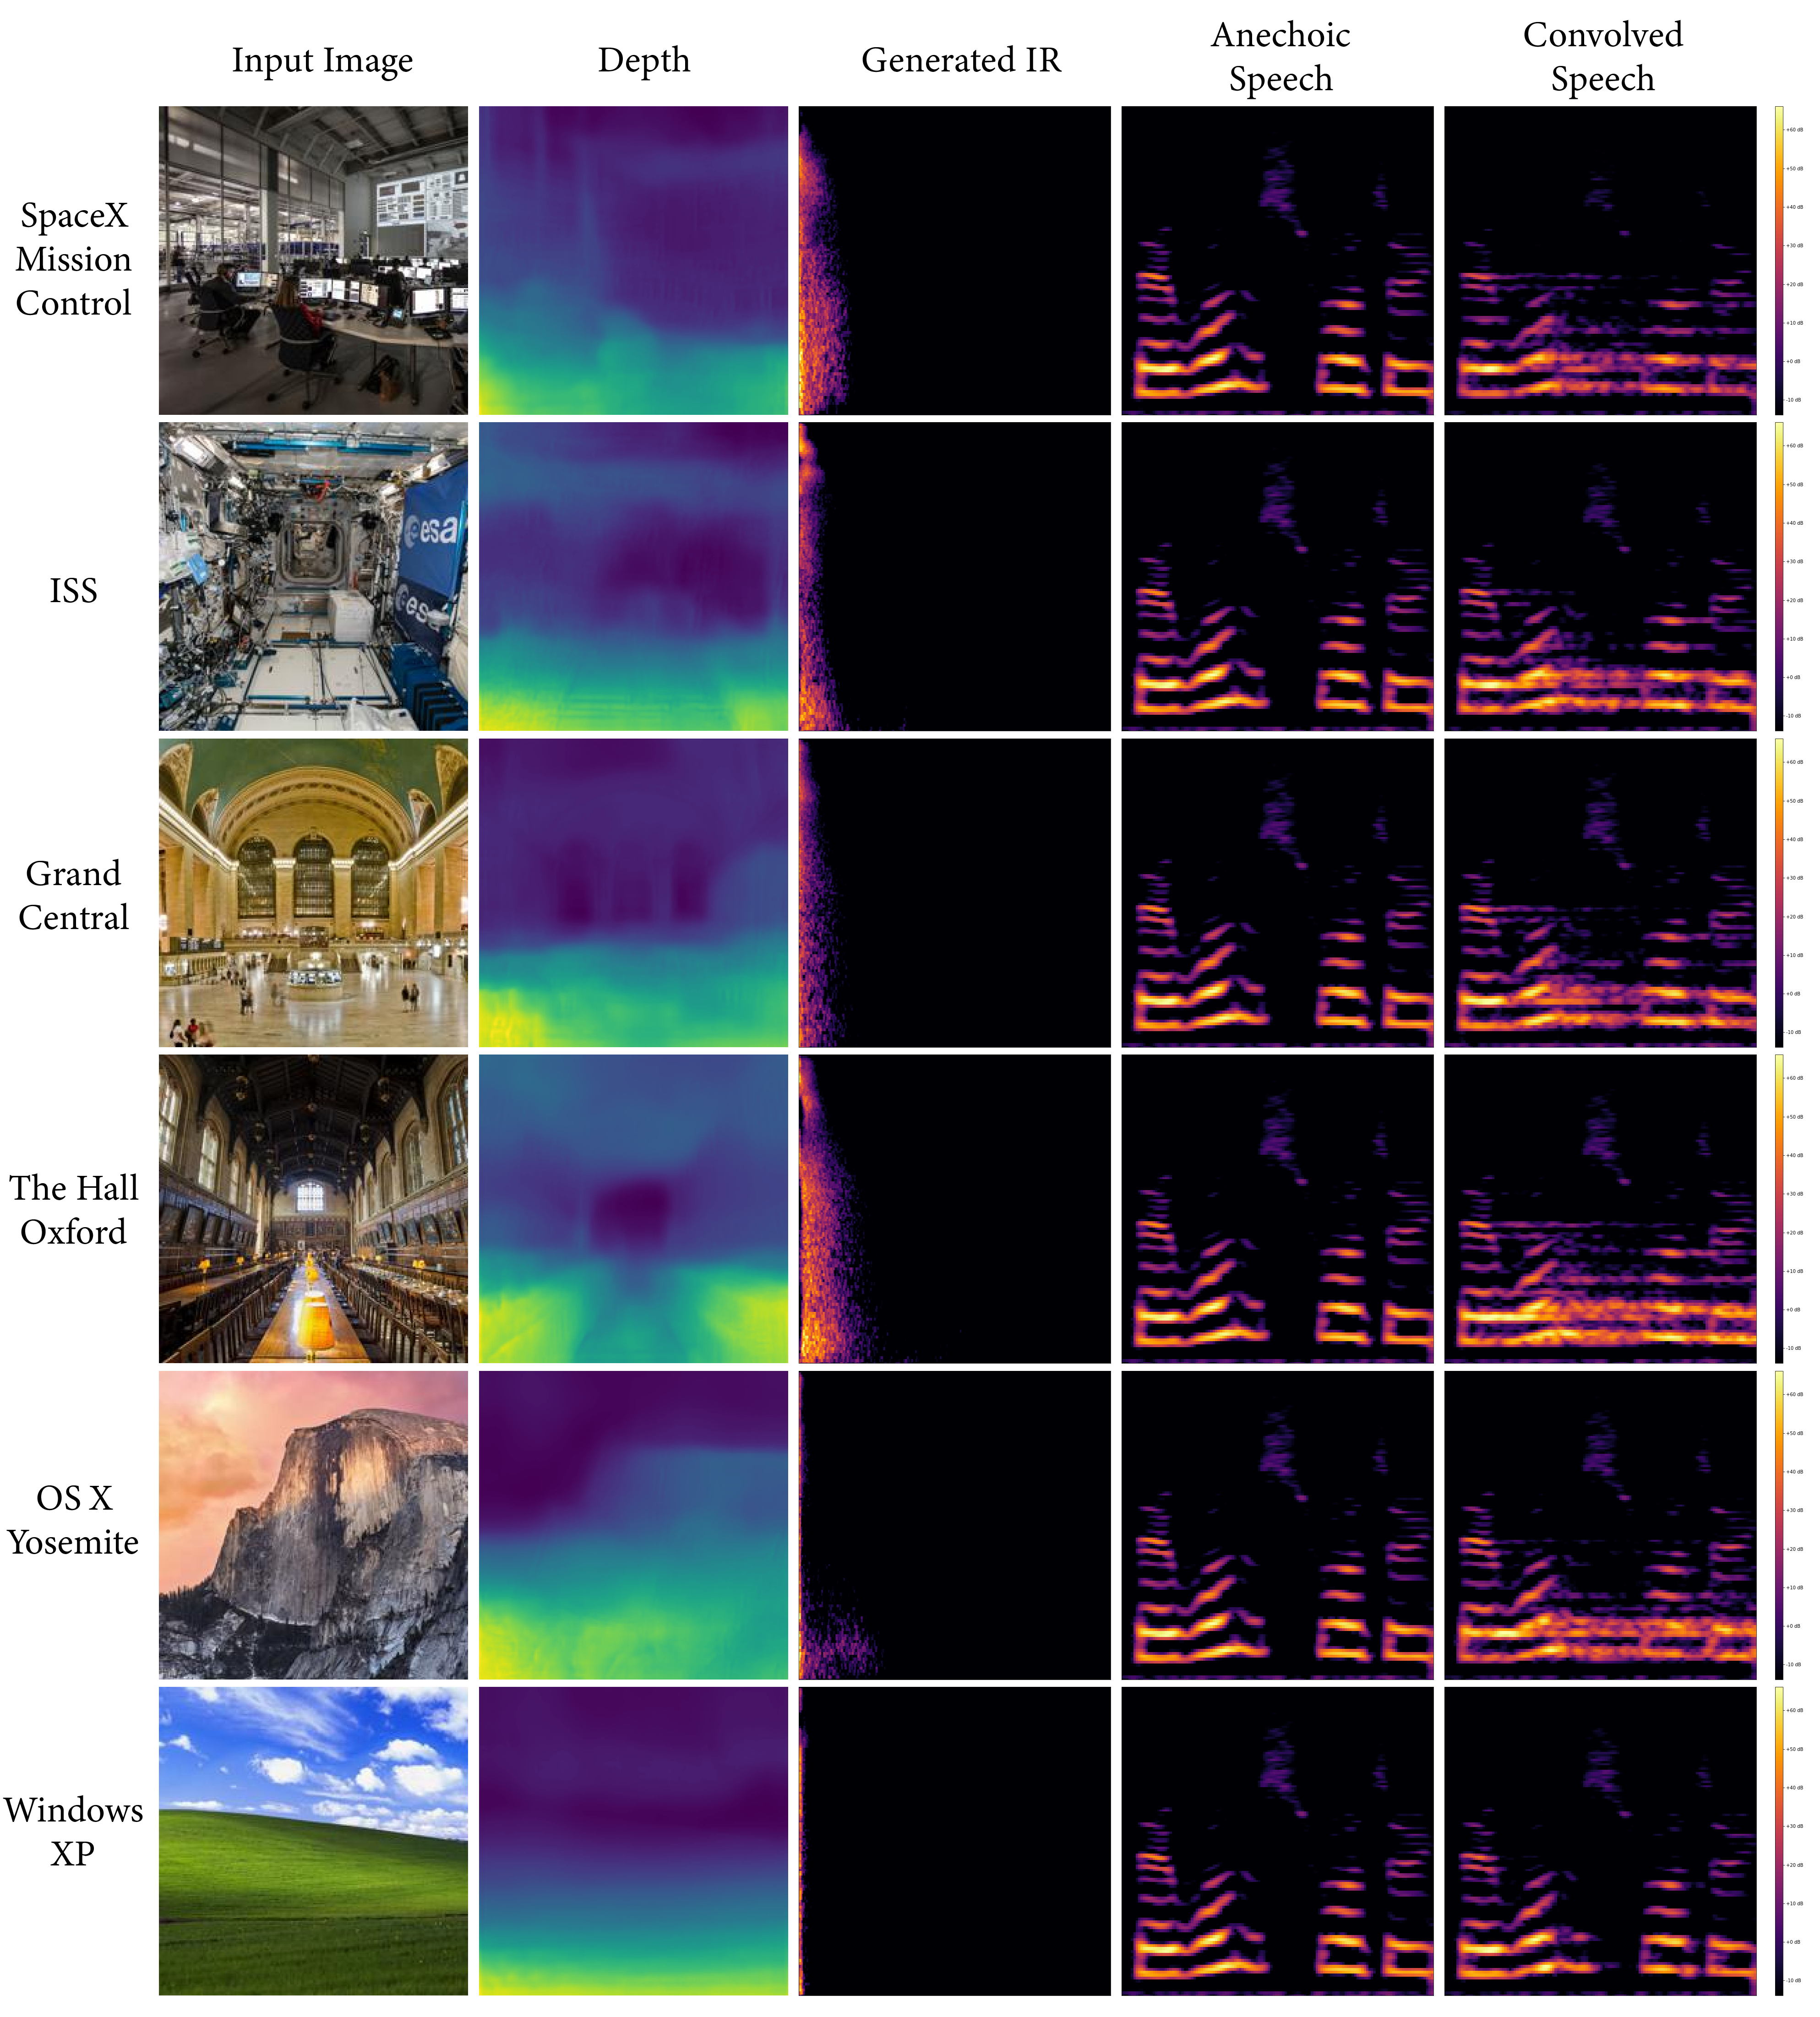
\includegraphics[width=0.9\textwidth]{p_famous.png}
    \caption{Famous and iconic spaces. Columns show input images, depth maps, generated IRs, and a dry anechoic speech signal before and after the generated IR was applied to the signal via convolution. The input images come from spaces that may be impractical or impossible to record in. The indoor spaces here show longer impulse responses compared to the outdoor scenes which is typically observed and expected in real-world settings. Larger indoor spaces also tend to exhibit greater $T_{60}$ times with longer impulse responses which we see here, though the ISS image has a longer impulse response than we expect.}
    \label{fig:p_famous}
\end{figure*}

\begin{figure*}
    \centering
    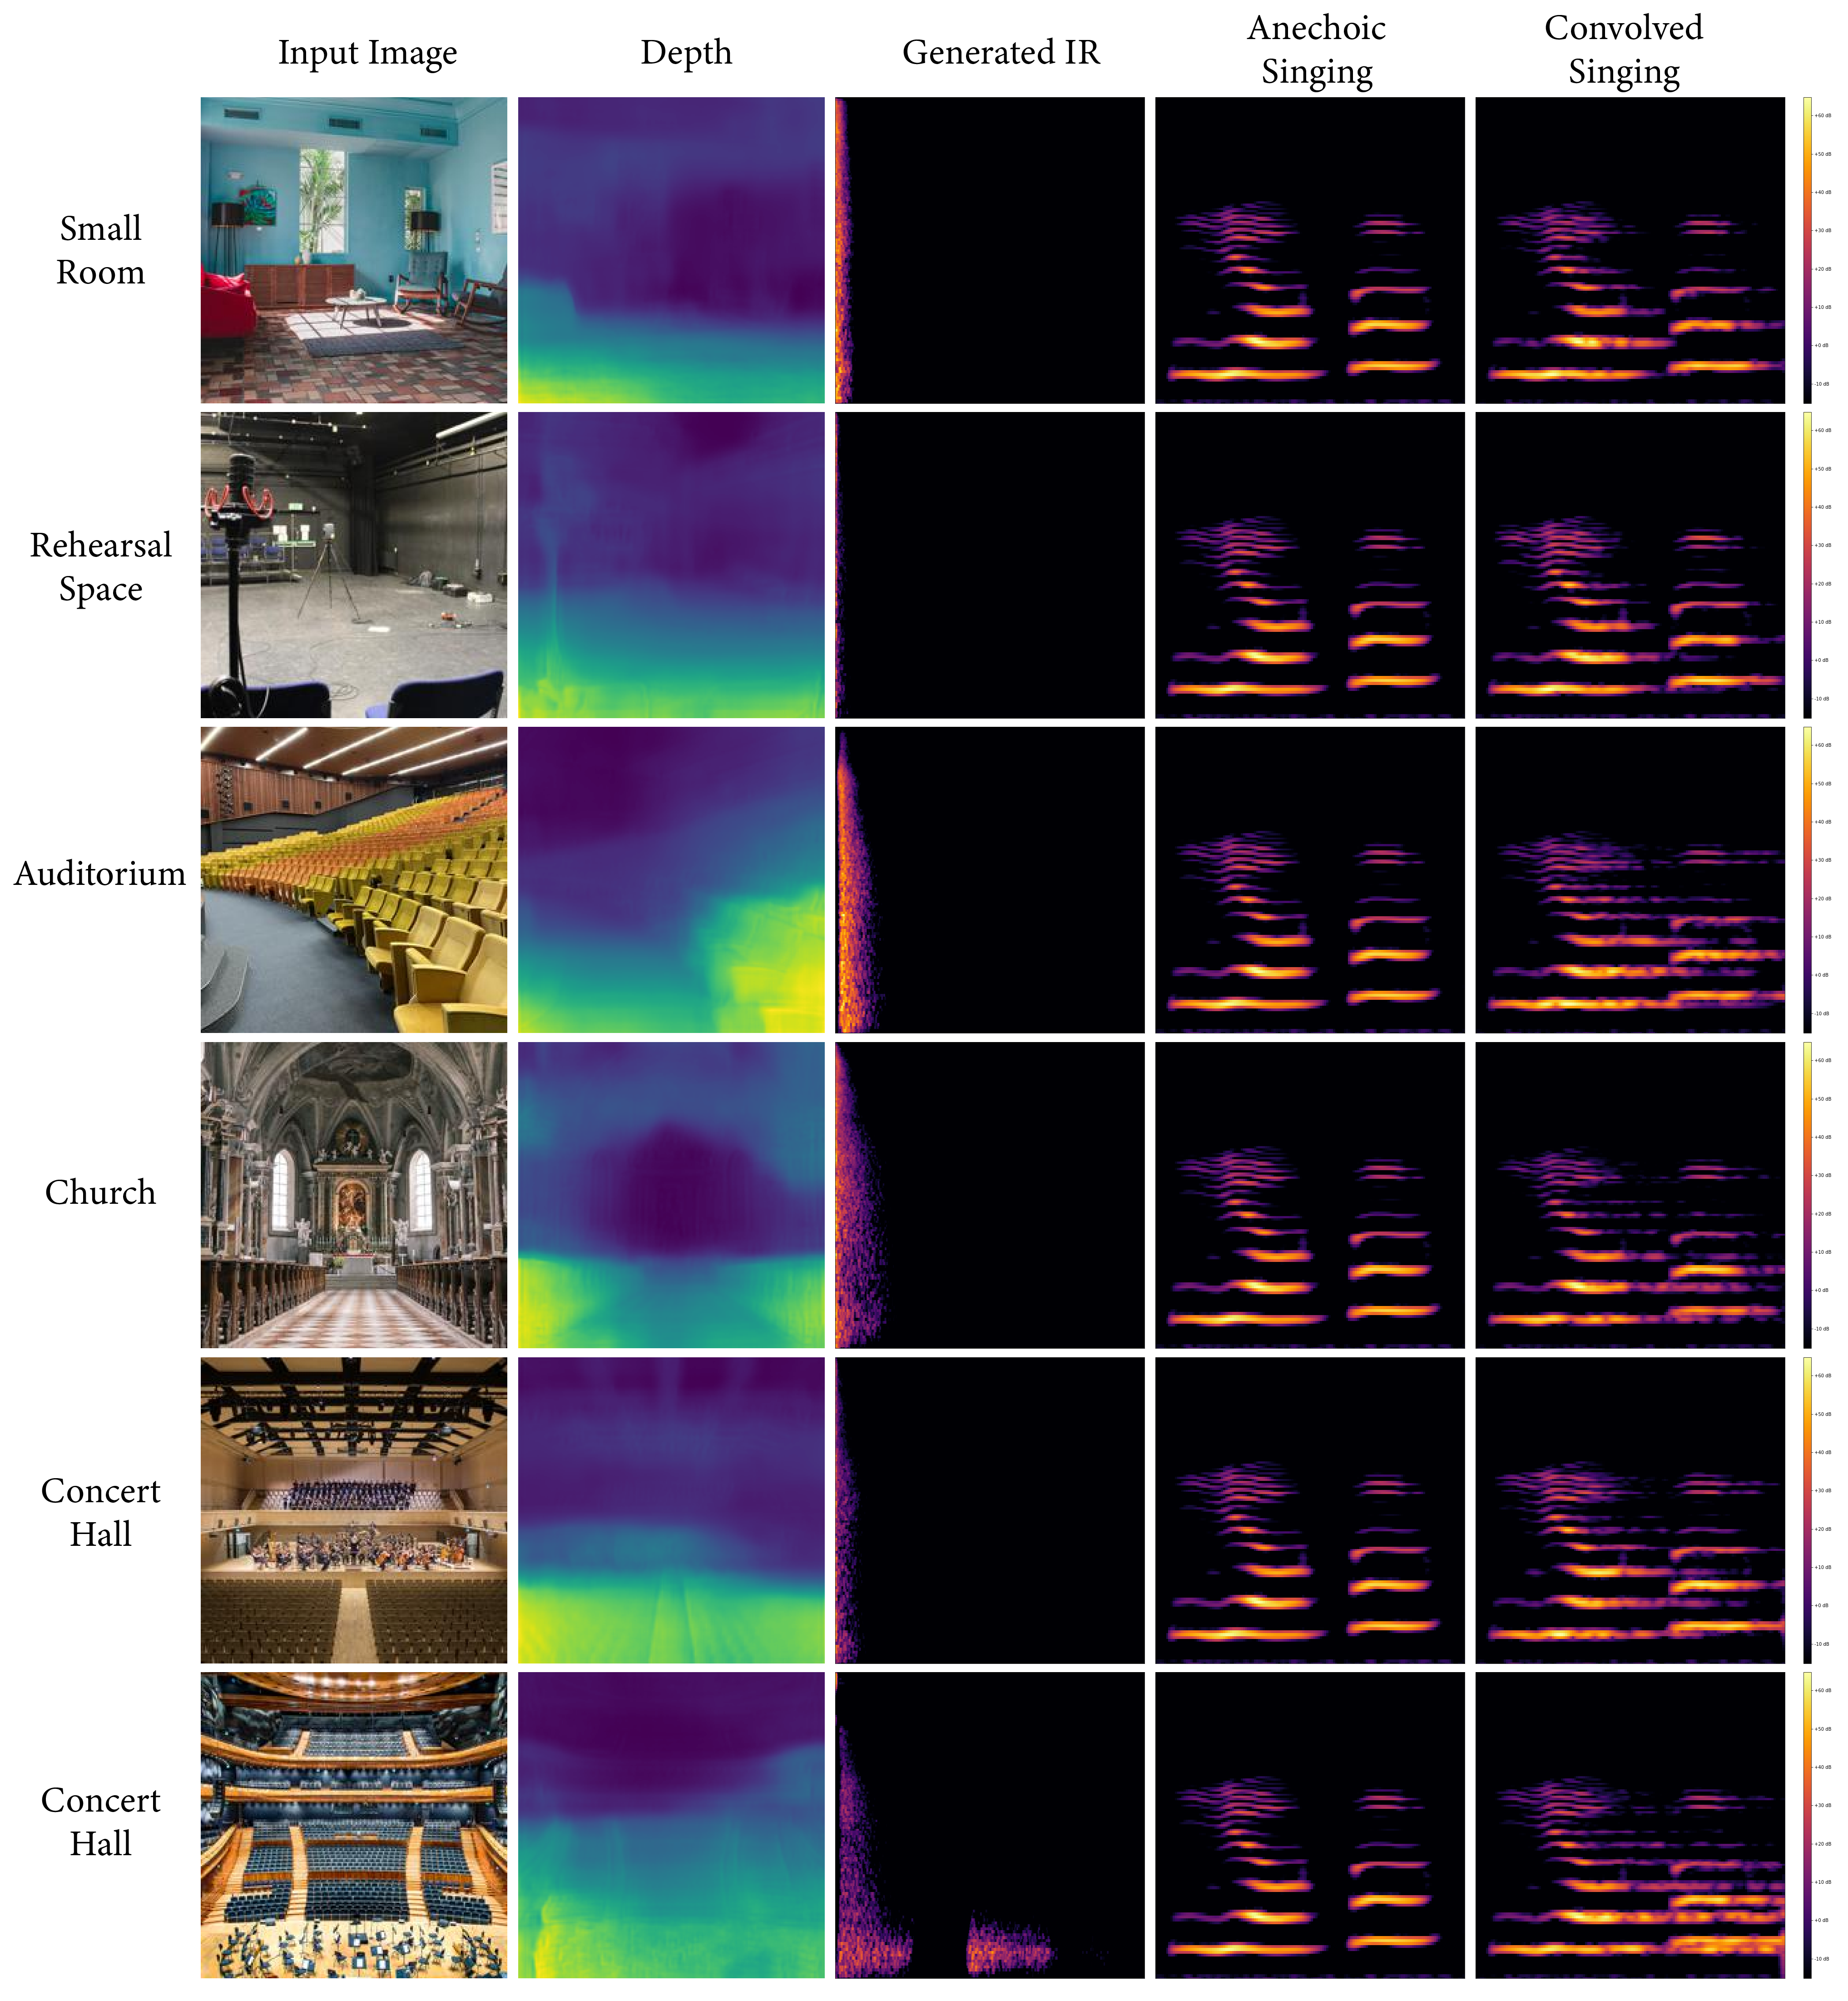
\includegraphics[width=0.9\textwidth]{p_music.png}
    \caption{Music. Columns show input images, depth maps, generated IRs, and an anechoic vocal singing signal before and after the generated IR was applied to the signal via convolution. The input images come from spaces relevant to music including a typical small room, an acoustically treated rehearsal space, an auditorium, a church, and 2 large concert halls. Generally, larger spaces tend to exhibit longer decay times in the output, however some examples such as the concert halls with visible acoustic treatment appear to have a shorter decay than more reverberant spaces like the church or auditorium with more reflective surfaces. The final concert hall shows an atypical impulse response with a visible discontinuity in the IR tail. This is not commonly observed among our model outputs, but illustrates the nature of artifacts which can occasionally occur.}
    \label{fig:p_music}
\end{figure*}

\begin{figure*}
    \centering
    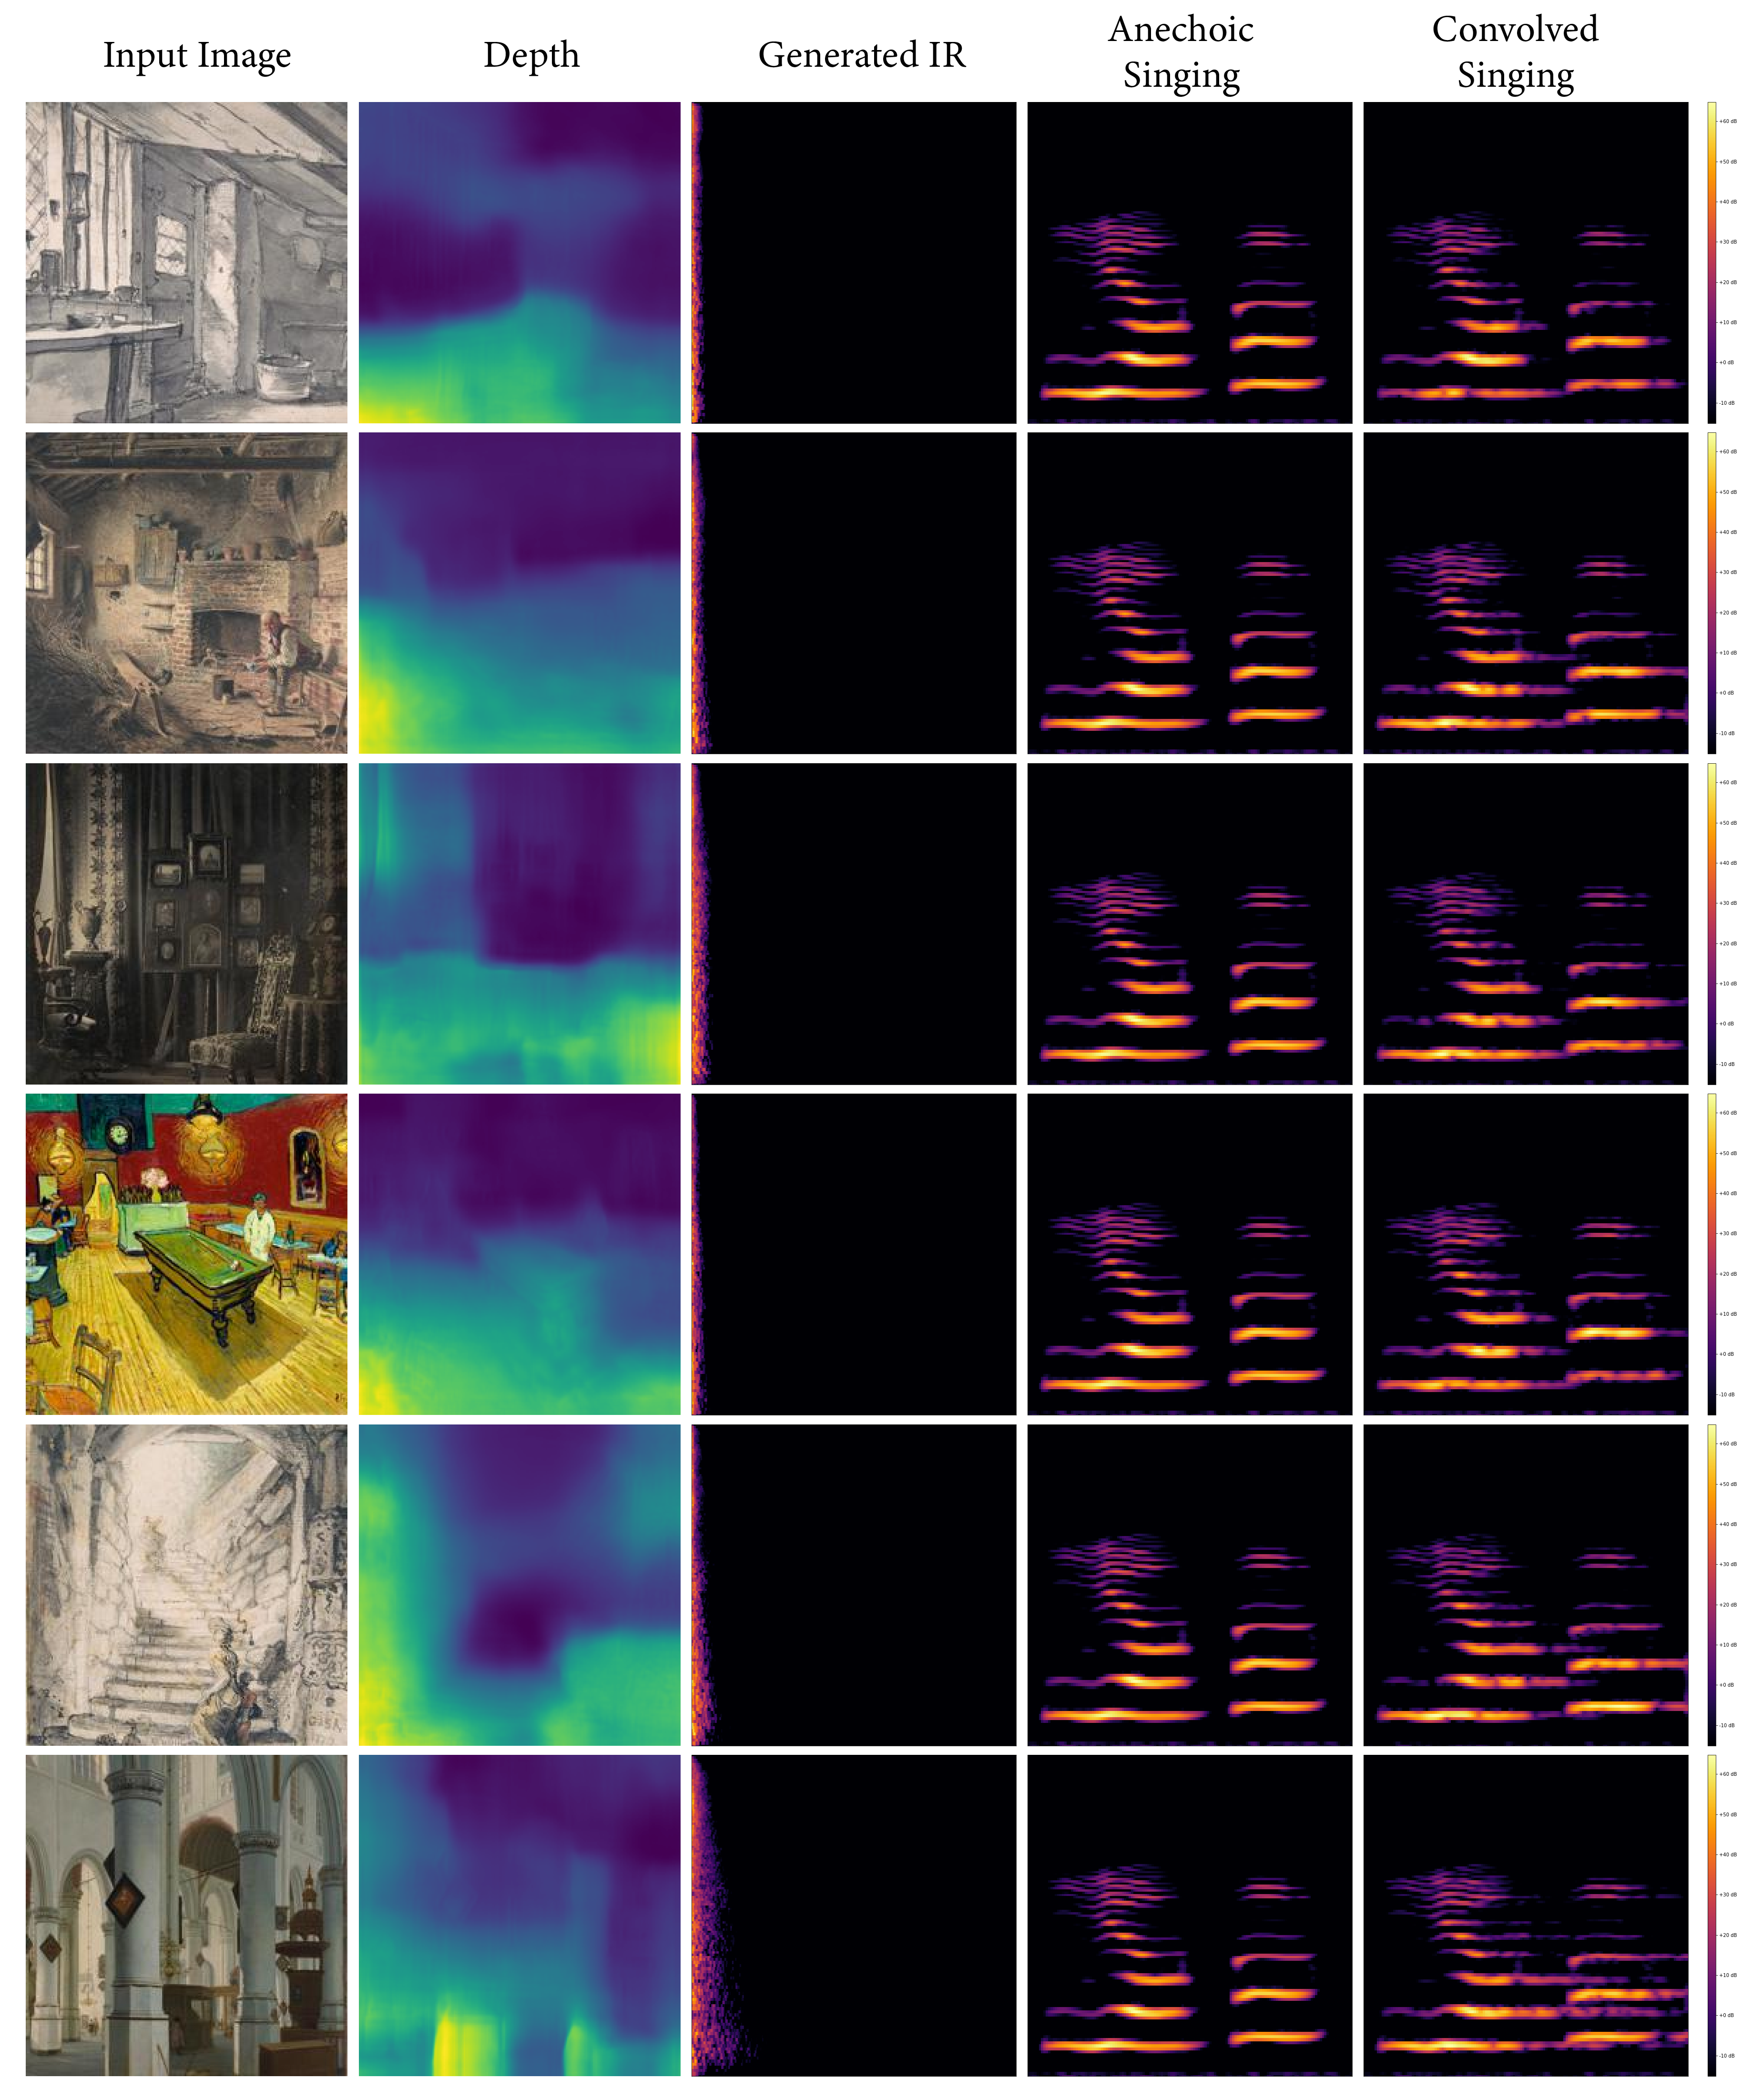
\includegraphics[width=0.82\textwidth]{p_art.png}
    \caption{Art. Columns show input images, depth maps, generated IRs, and an anechoic operatic singing signal before and after the generated IR was applied to the signal via convolution. Images here are drawings, paintings and a vintage art photograph ca. 1850. Artistic depictions of spaces were not included in our training dataset. In many cases, plausible impulse responses are generated from such input images. In general, larger depicted spaces, like the church in the bottom row, exhibit longer decay times as is observed with standard 2D photographs.}
    \label{fig:p_art}
\end{figure*}

\begin{figure*}
    \centering
    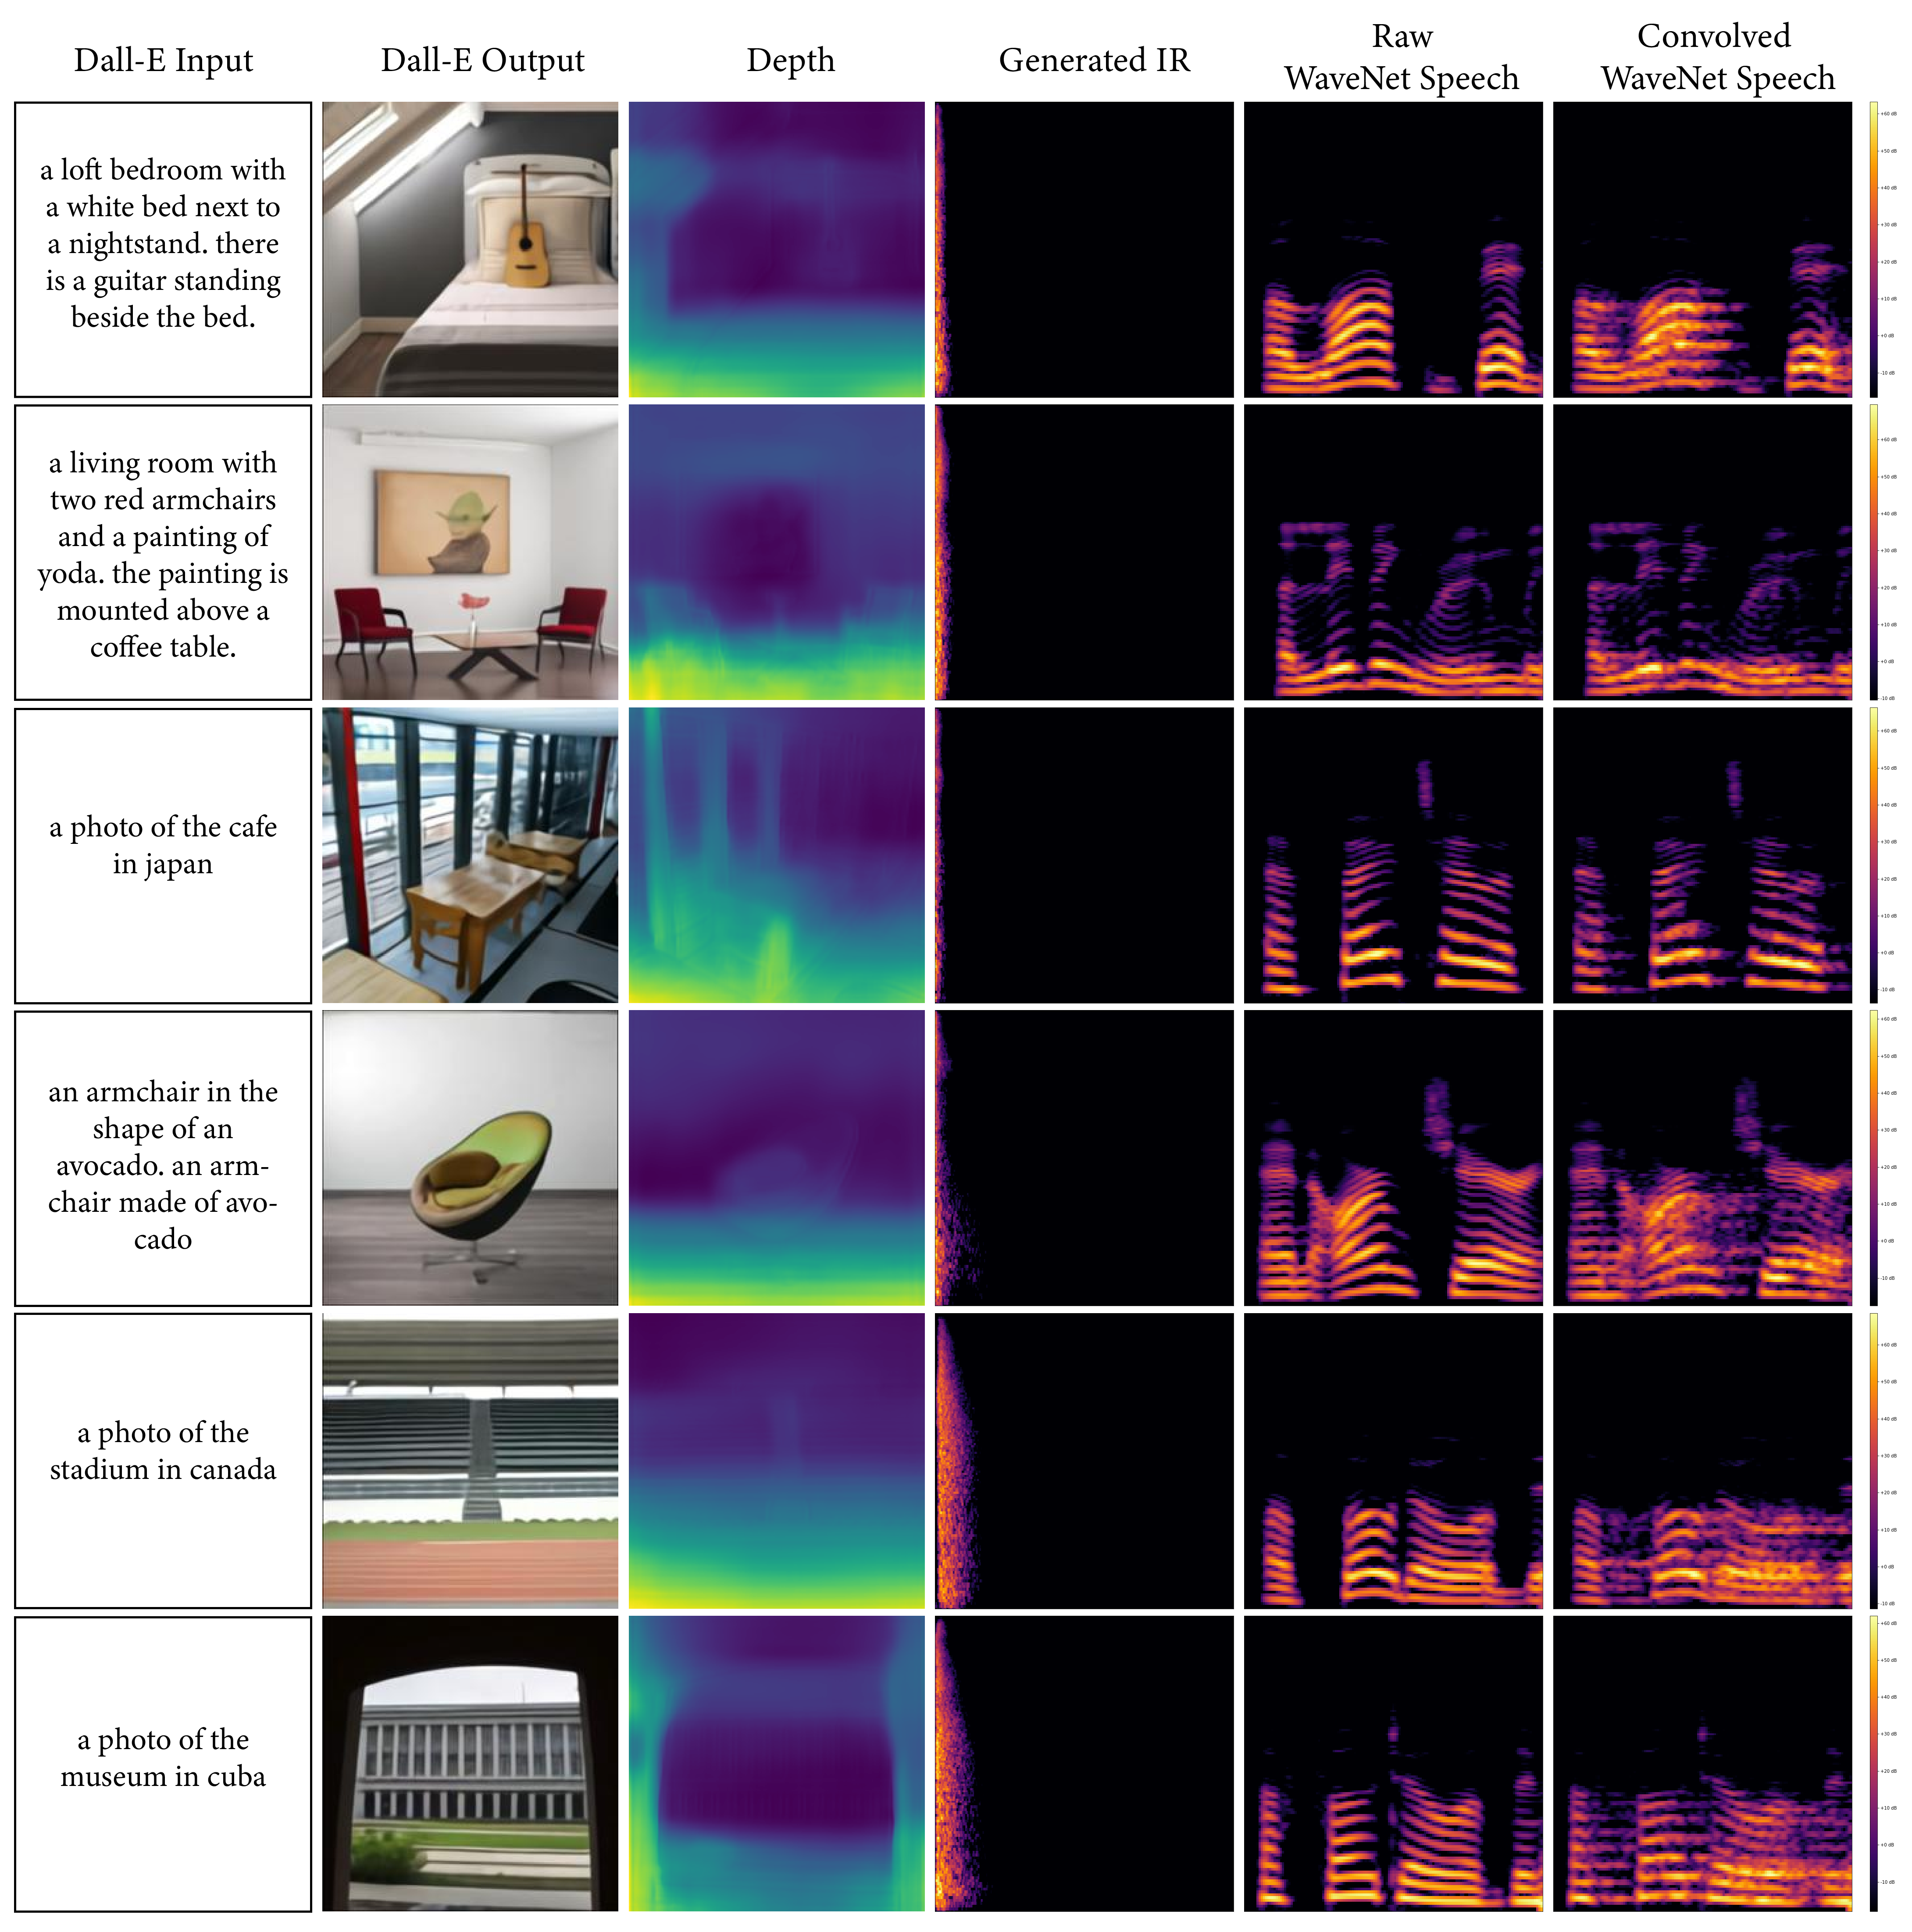
\includegraphics[width=\textwidth]{p_dall-e.png}
    \caption{DALL·E. Images generated from text by DALL·E \cite{dalle} used here as input images. The same corresponding input text was synthesized via text-to-speech as our signal of interest and convolved with the generated IR.  This reflects synthetic speech in a synthetic environment, indicating a path for synthesizing realistic IRs from text. It also shows how our model might work with other state-of-the-art generative media models to produce more consistent and realistic results in different domains.}
    \label{fig:p_dall-e}
\end{figure*}

\begin{figure*}
    \centering
    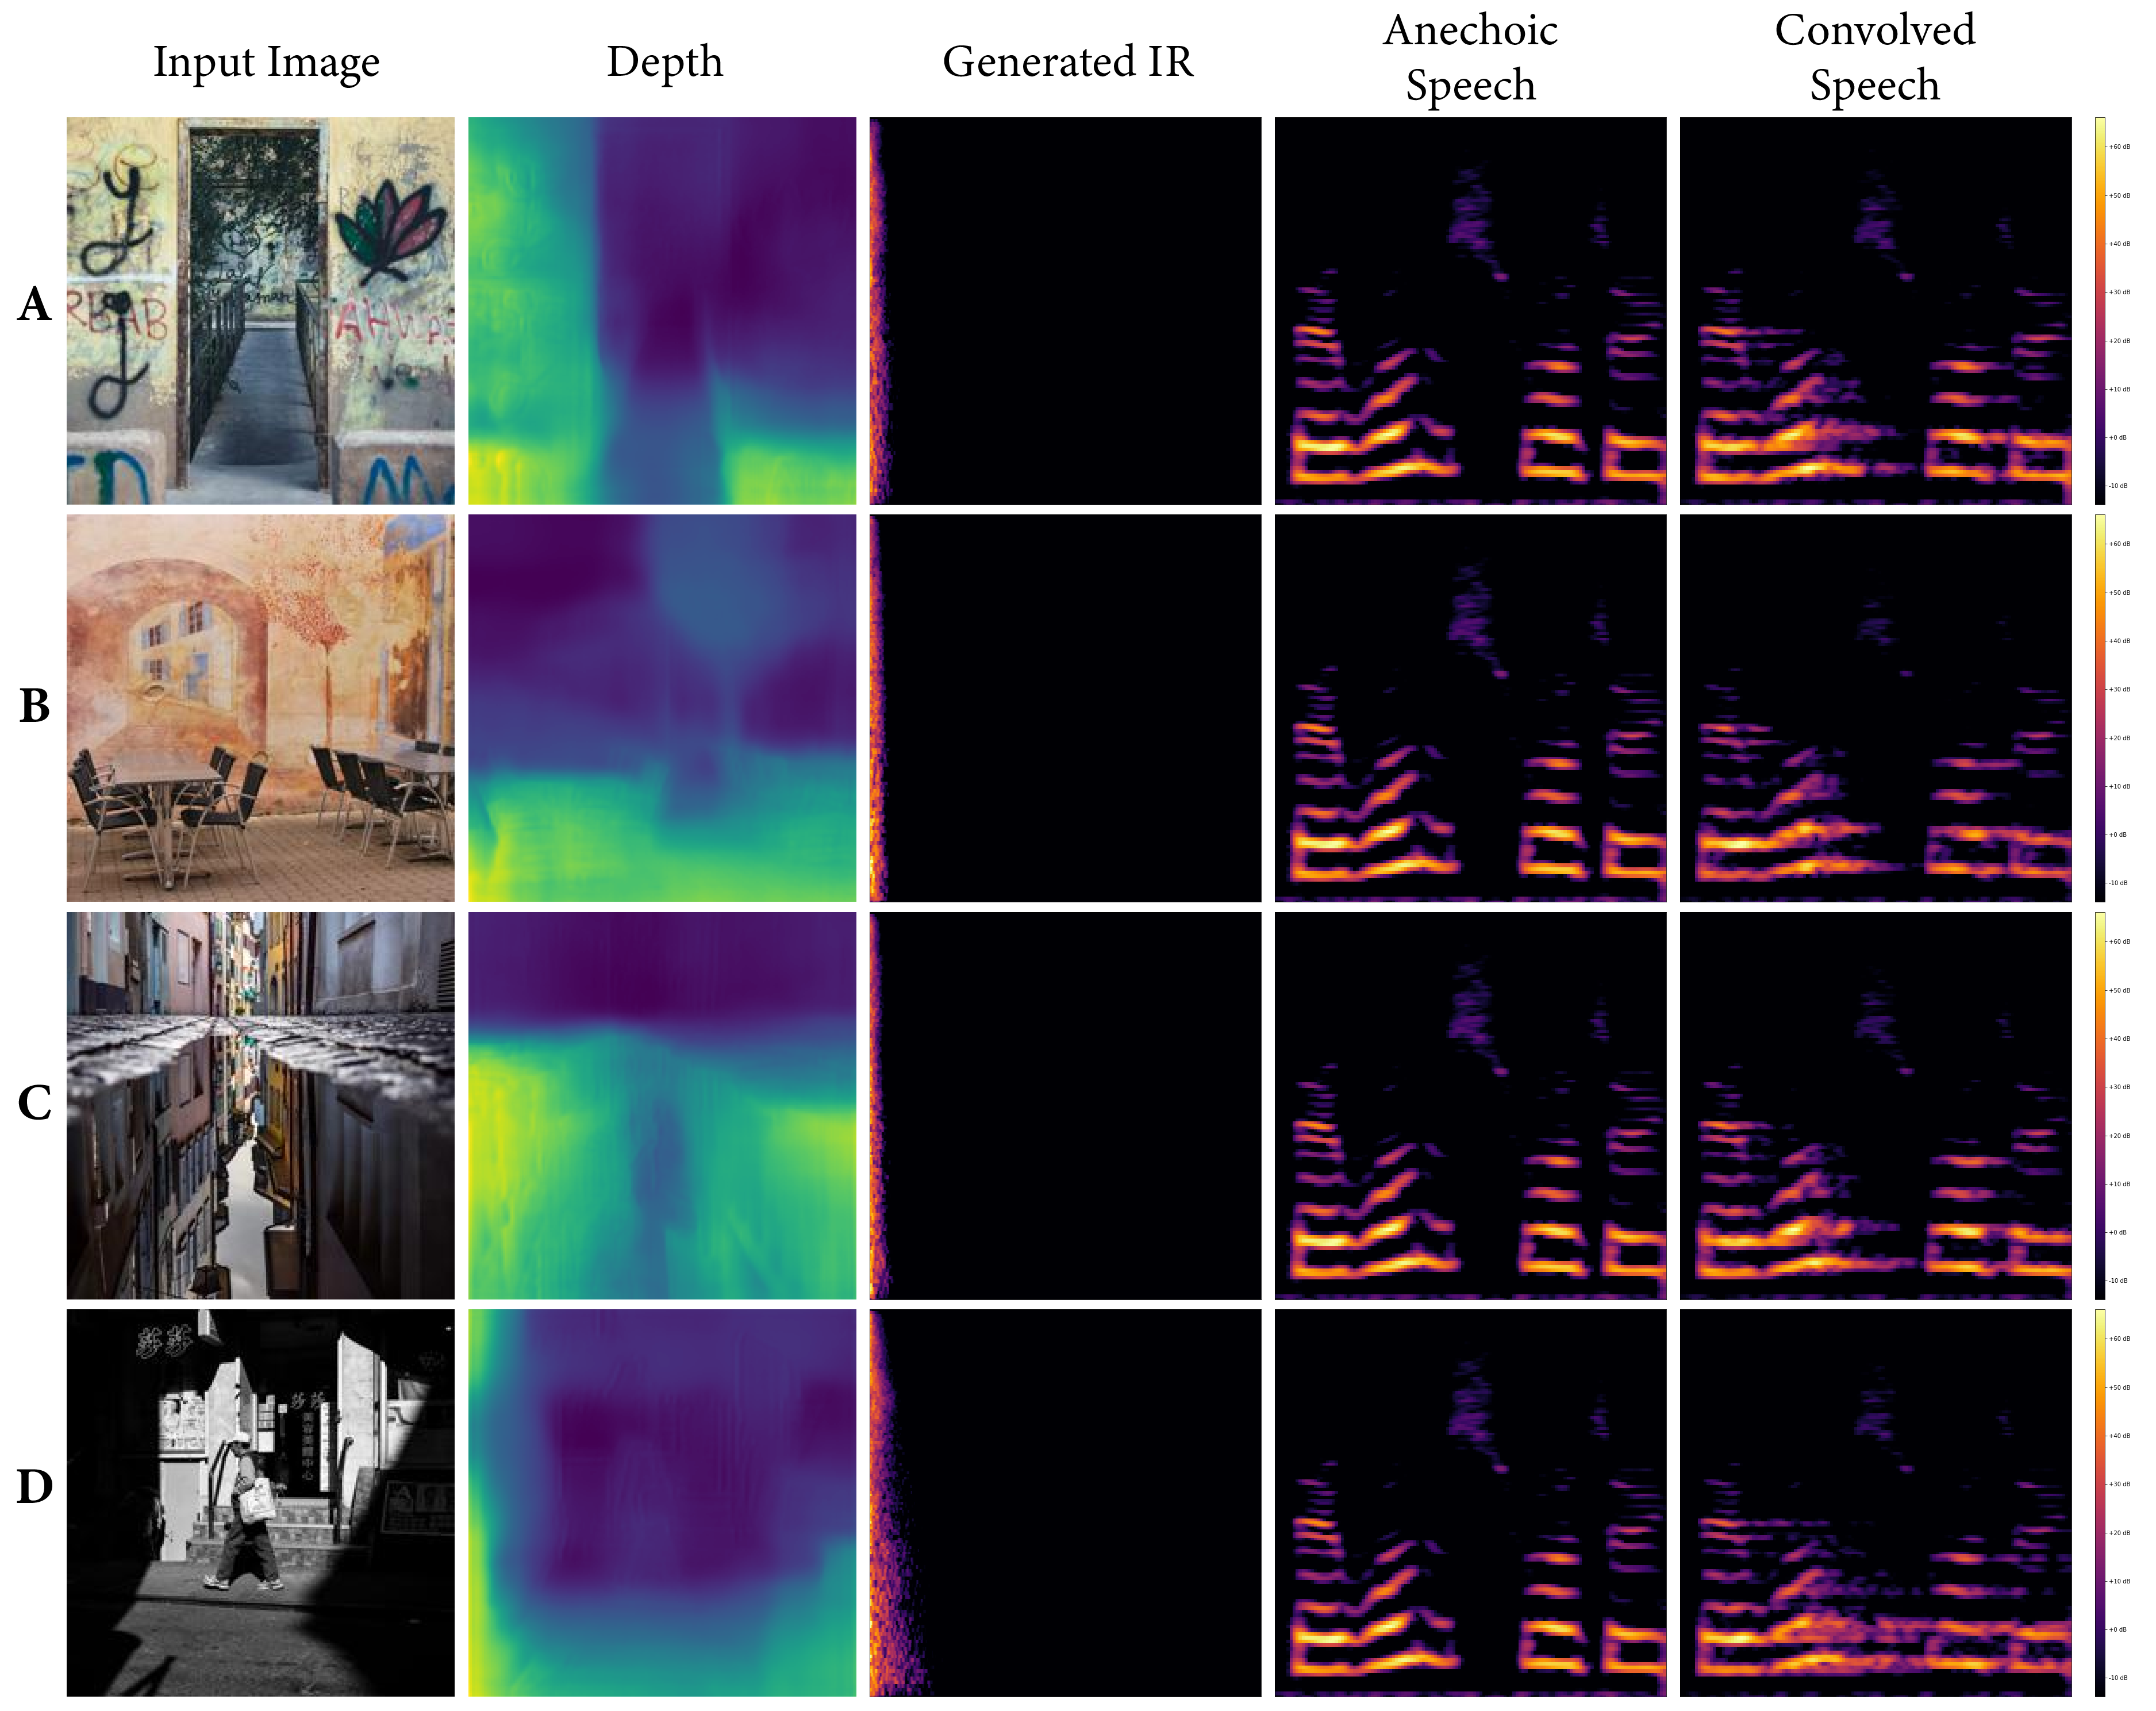
\includegraphics[width=0.85\textwidth]{p_reflection.png}
    \caption{Challenging images. Input images containing street murals, reflections, and shadows demonstrating cases where depth is inaccurately estimated. (A) A painted doorway giving the illusion of depth. (B) A wall with a mural of a street and tree where the depth of the wall is inaccurately estimated. (C) A low-angle photo of a reflective puddle. (D) An outdoor street image with strong shadows which results in a depth map and generated IR more similar to a room than an outdoor space. These more extreme scenarios are chosen to clearly illustrate the limitations of our approach.}
    \label{fig:p_reflection}
\end{figure*}

\begin{figure*}
    \centering
    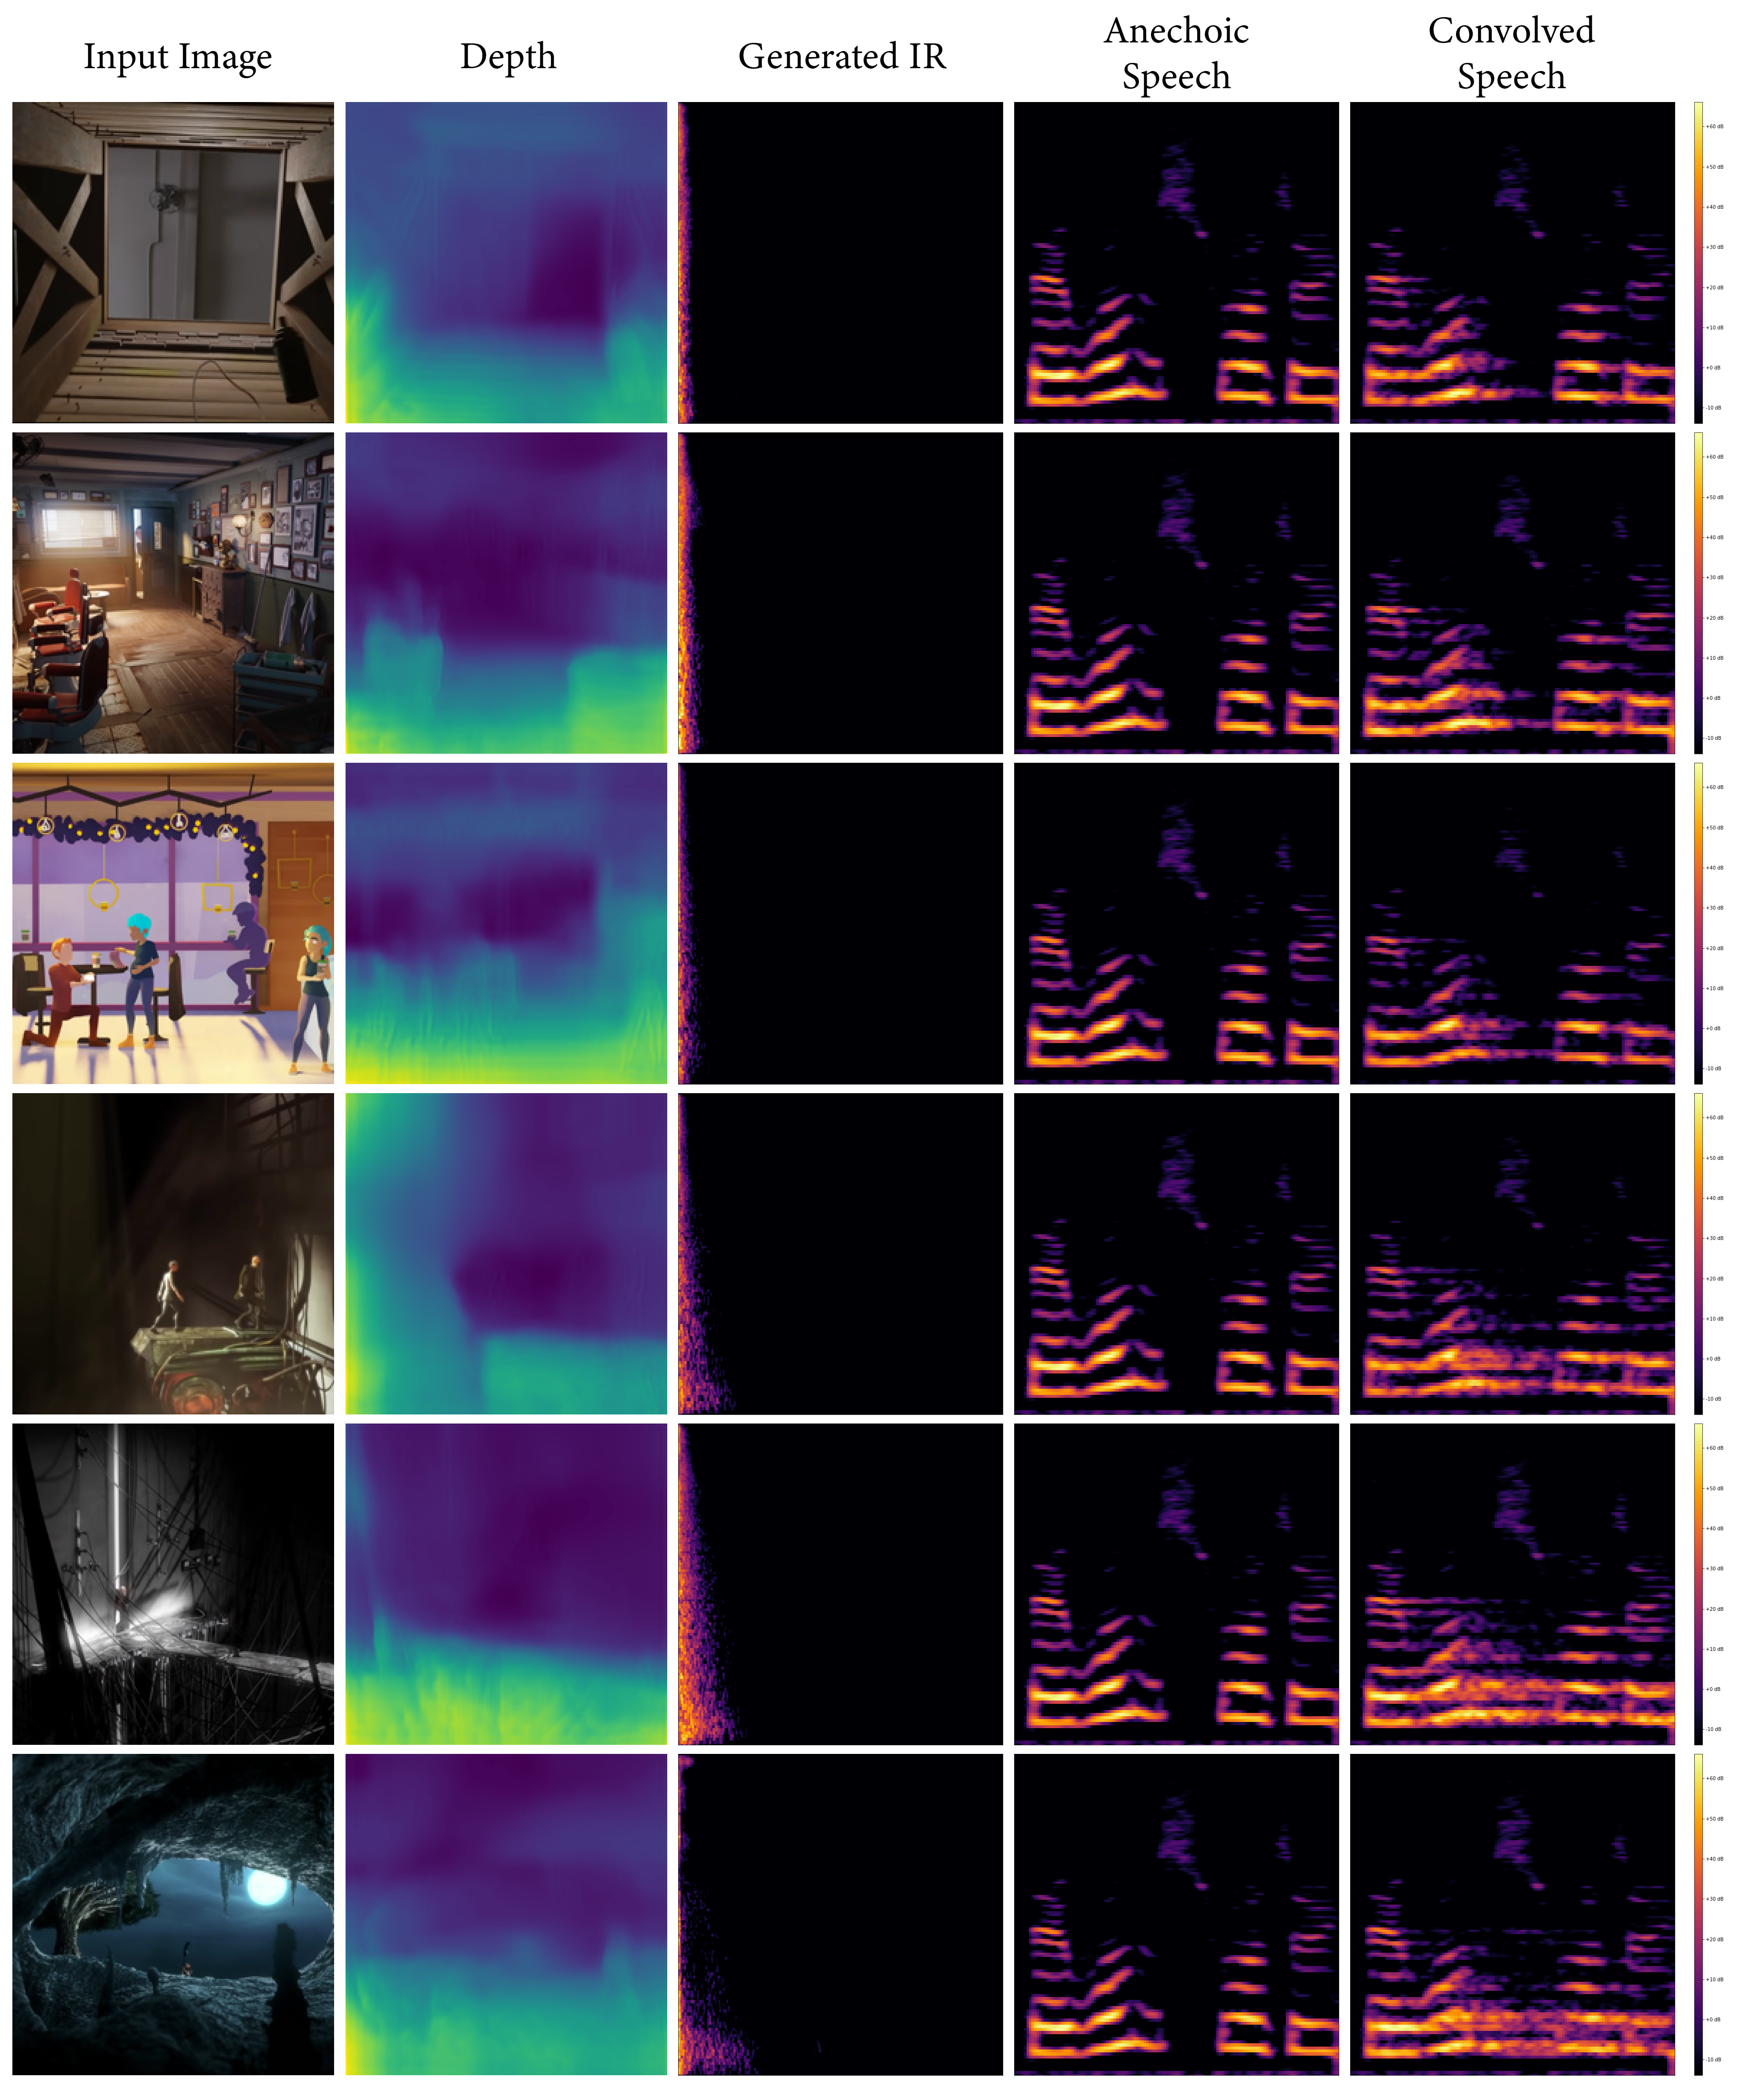
\includegraphics[width=0.85\textwidth]{p_animation.png}
    \caption{Animated films. Scenes from Blender open animation films used as input images (speech convolved with generated IRs). Columns show input image, calculated depth map, spectrogram of generated IR, an anechoic passage reading sample, and the same passage with the generated IR applied via convolution. In general, we find that our model plausibly estimates the reverberant characteristics of these spaces. For example, the wooden small space is very brief. The barbershop appears longer due to some artefacts, but the broadband decay is relatively quick as can be heard in the audio. Seemingly larger spaces again correspond to longer IRs. This is a case of Real2Sim transfer, where we can approximate IRs directly that sound as measured IRs, but in virtual environments where this measurement is not possible.}
    \label{fig:p_animation}
\end{figure*}

\begin{figure*}
    \centering
    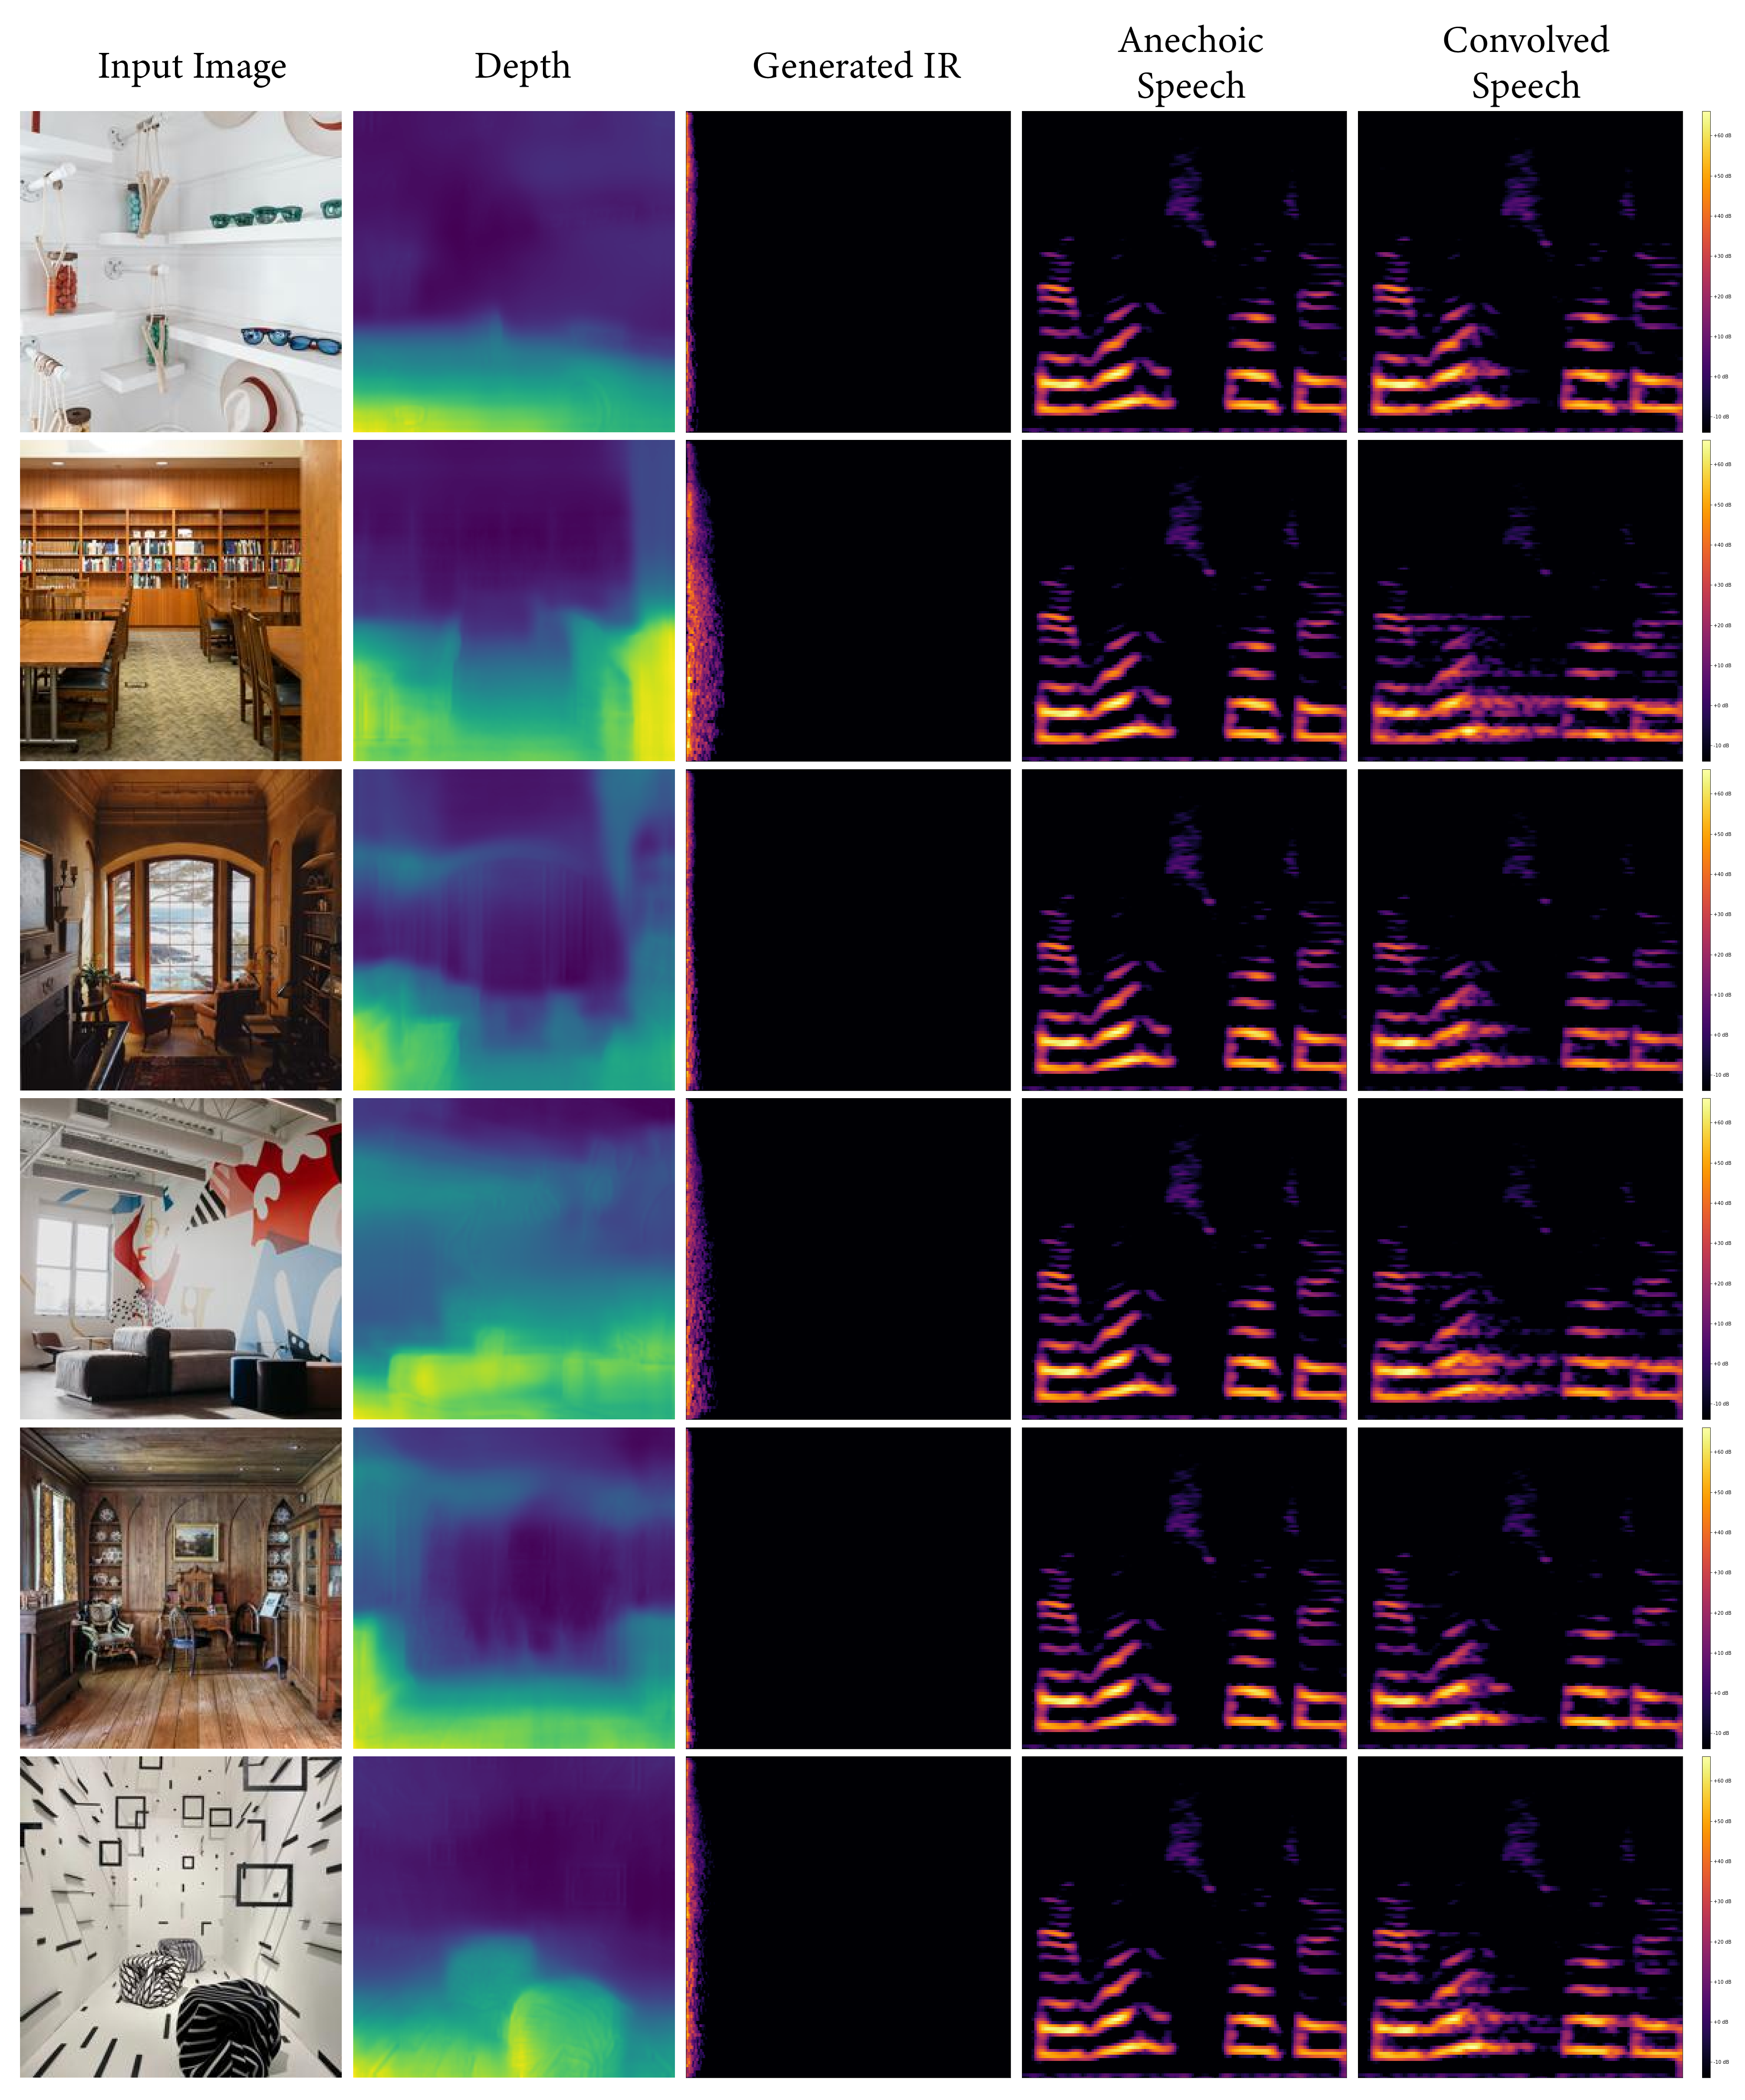
\includegraphics[width=0.85\textwidth]{p_zoom.png}
    \caption{Virtual backgrounds. Images which may serve as virtual backgrounds used as input images to our model. These reflect spaces that may be used for videoconferencing or other online meetings. Realistic IRs may be generated and used in these contexts to increase the sense of being in a shared space with others.}
    \label{fig:p_zoom}
\end{figure*}

\begin{figure*}
    \centering
    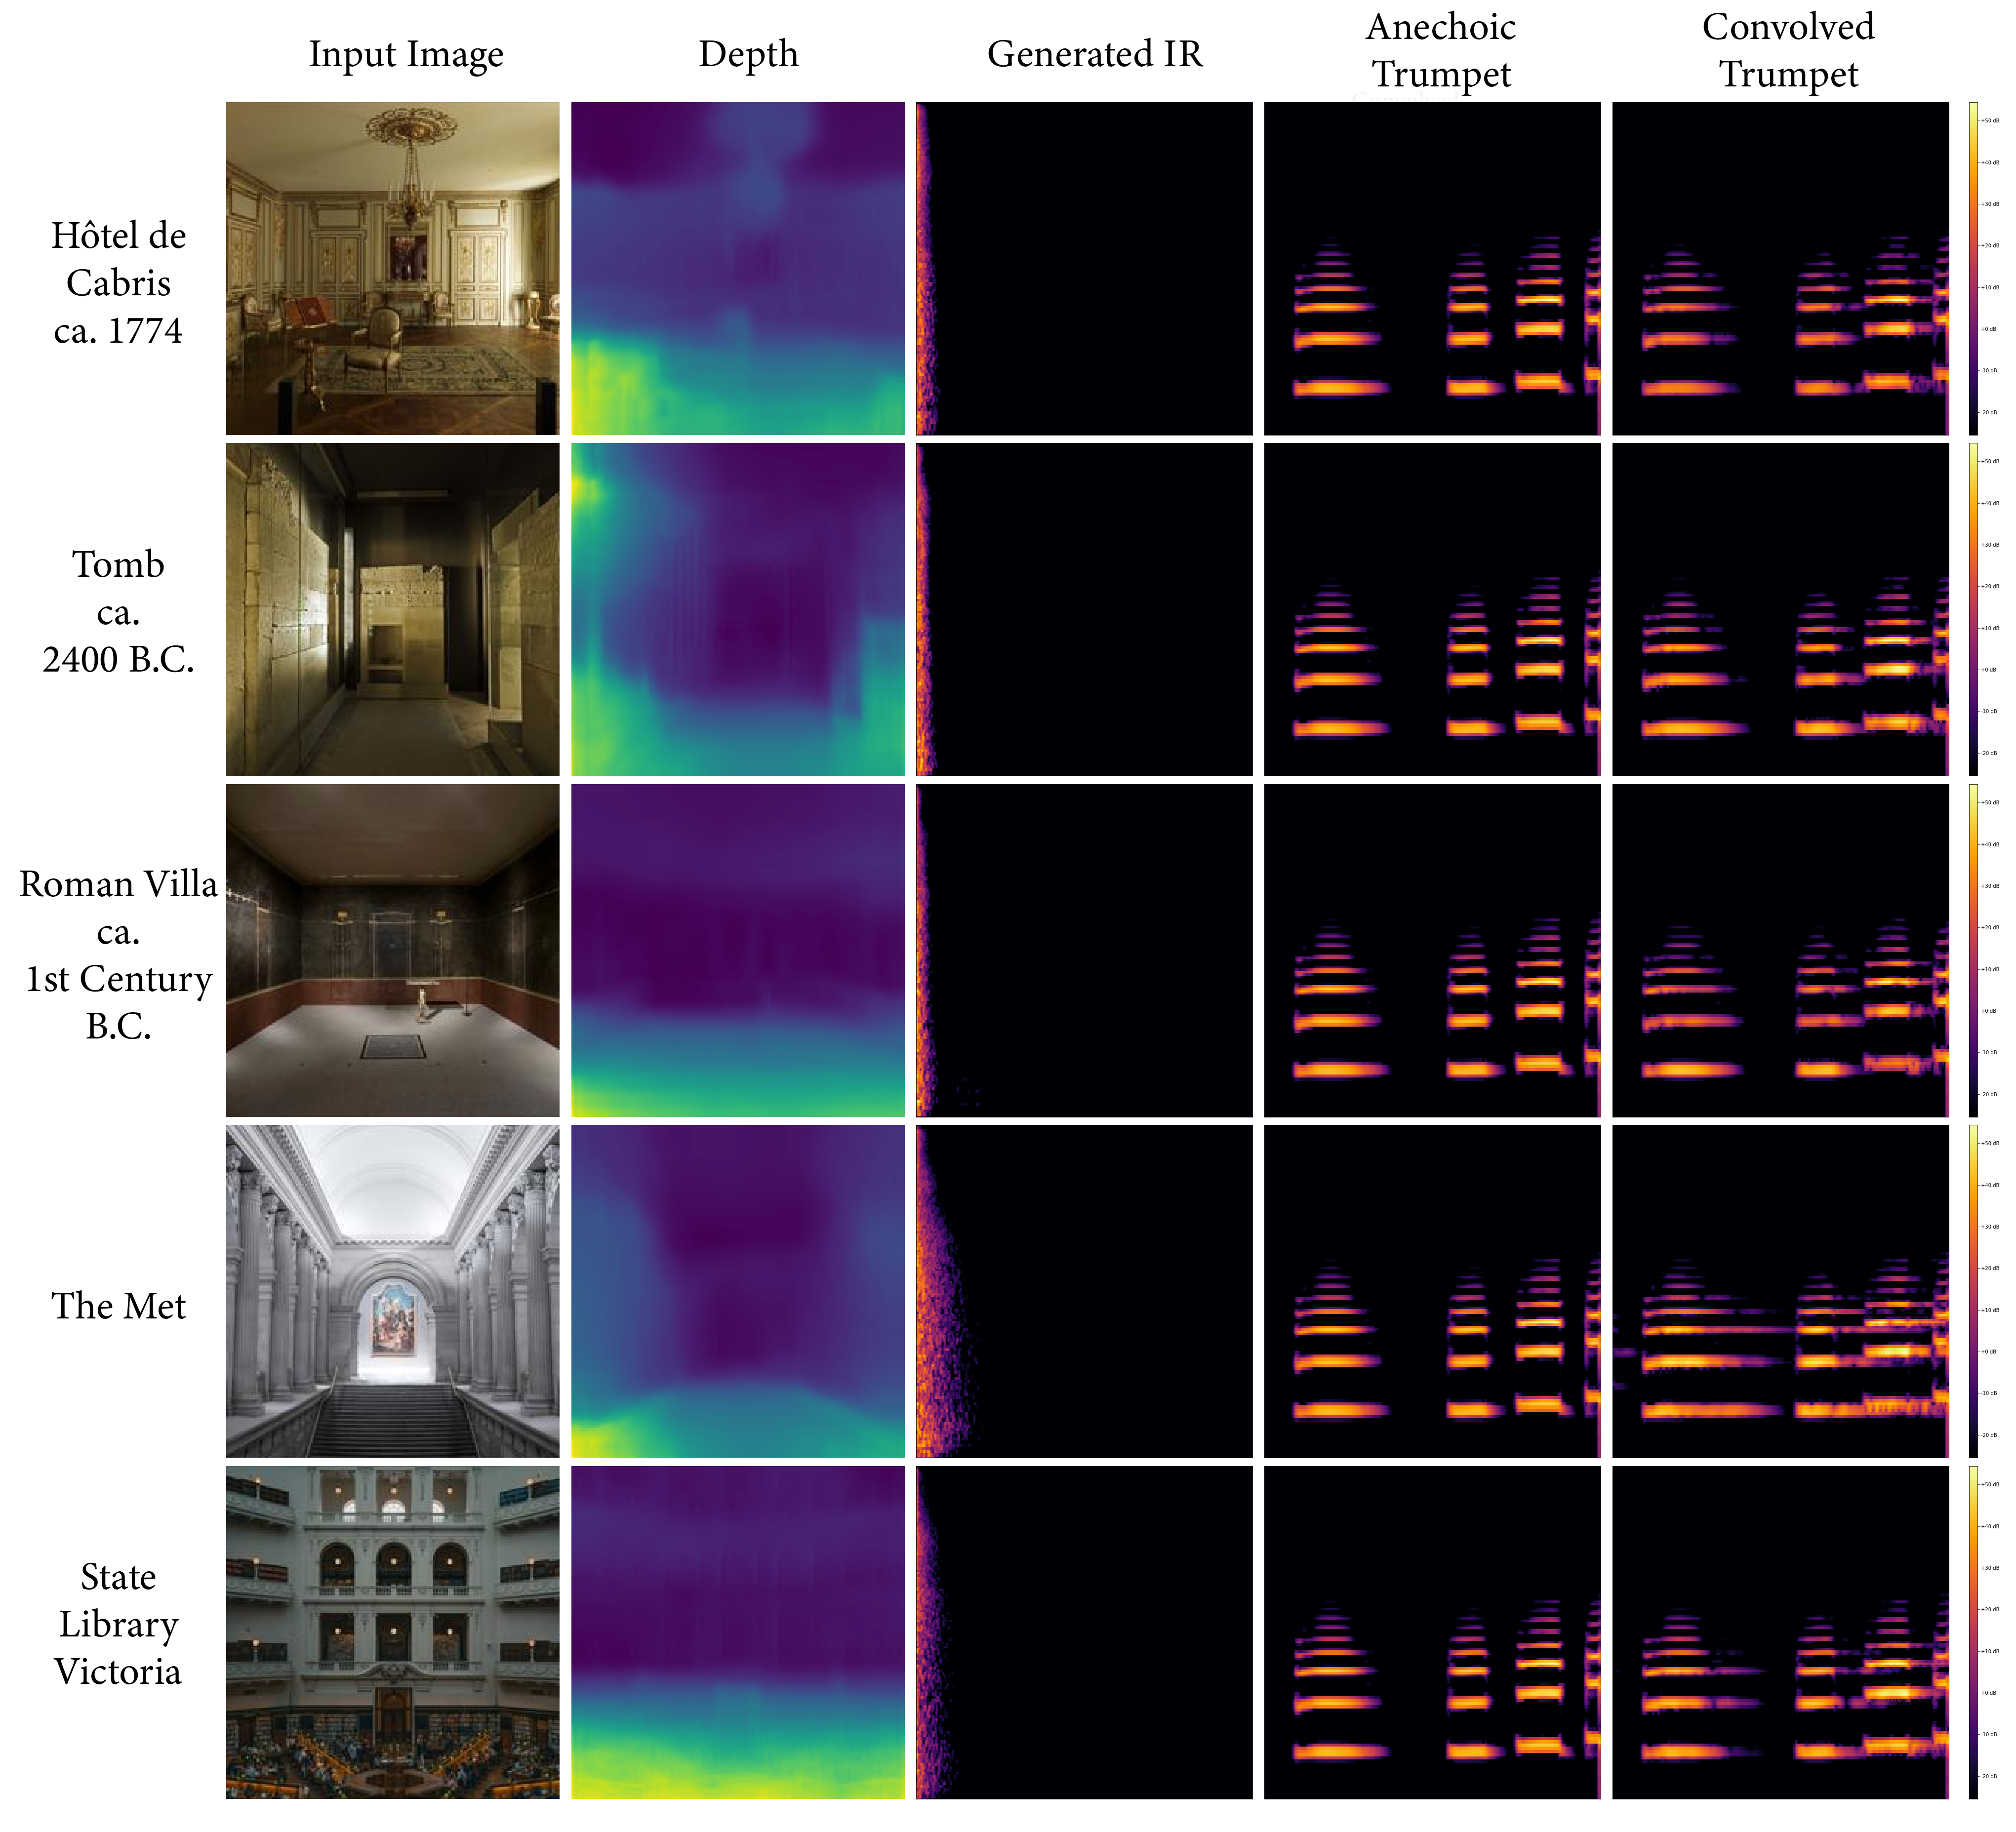
\includegraphics[width=0.9\textwidth]{p_other.png}
    \caption{Historical and notable places. Additional examples of unusual and historical spaces which may be difficult or impossible to obtain IRs from.}
    \label{fig:p_other}
\end{figure*}

\begin{figure*}
    \centering
    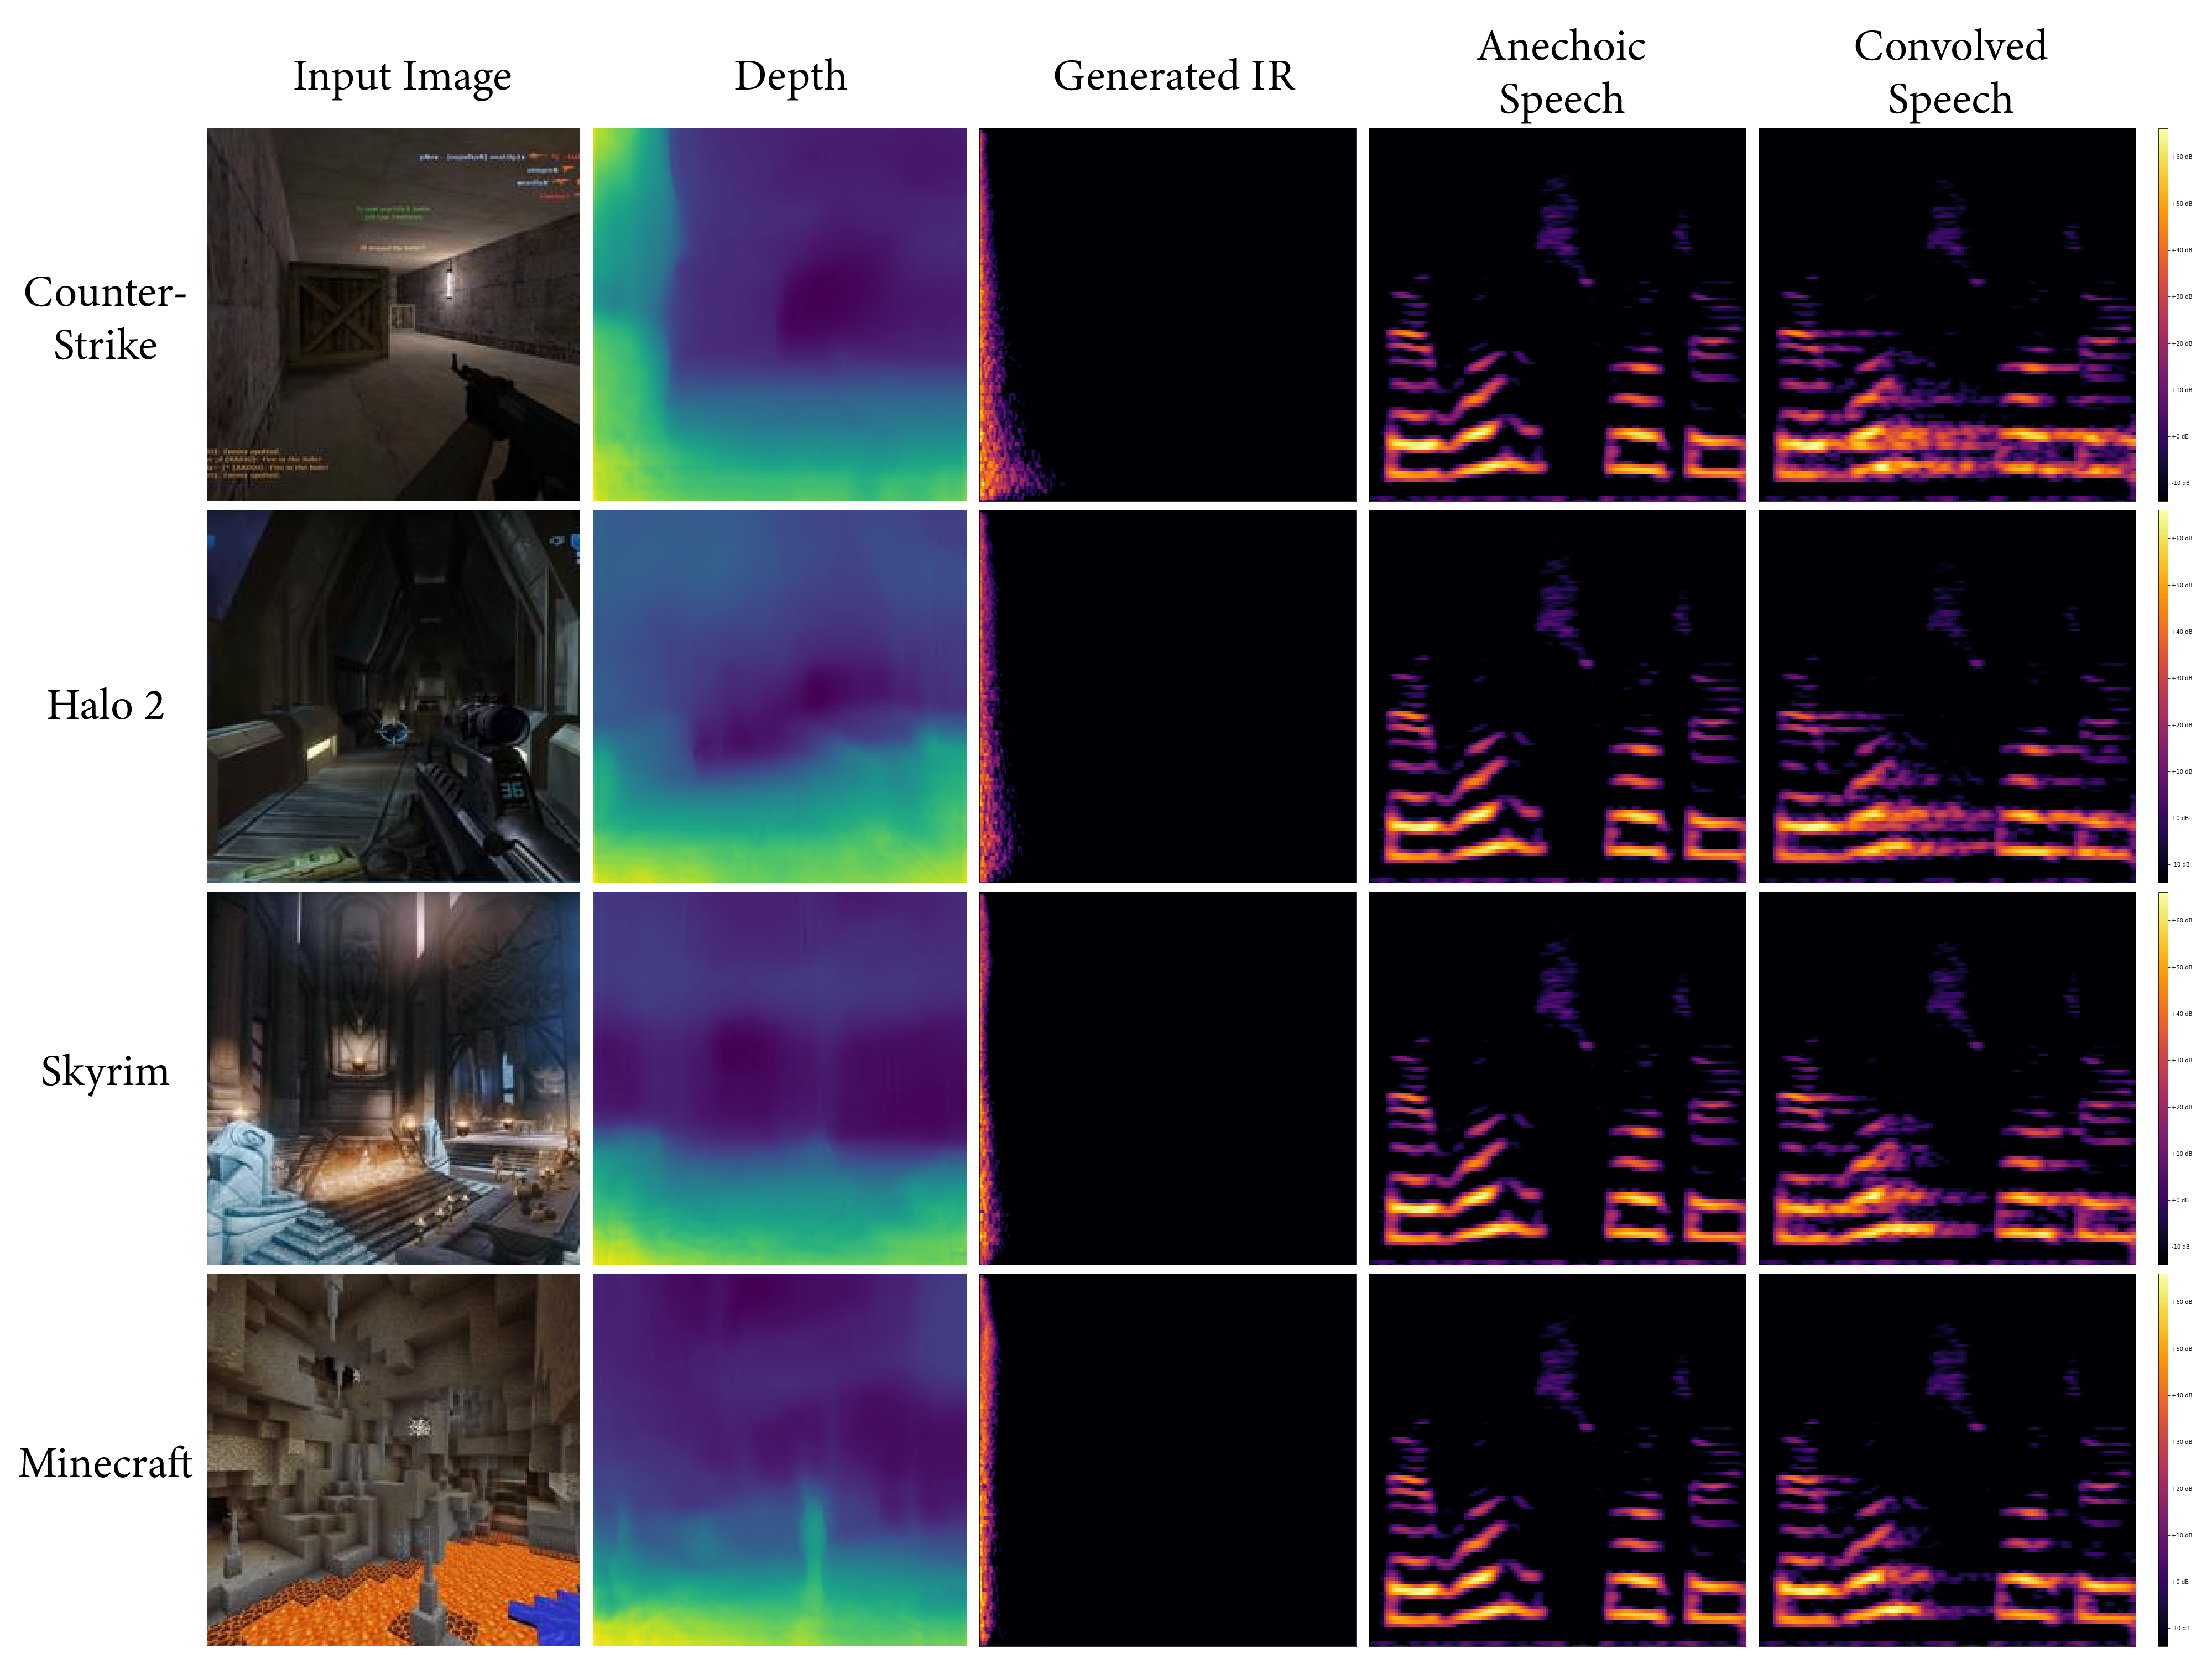
\includegraphics[width=0.9\textwidth]{p_videogame.png}
    \caption{Video games. Impulse responses generated and applied via convolution from screenshots of four 3D video games. Video games are one example of a virtual space that might benefit from easily generated impulse responses. While the medium sized room from Counter-Strike and the large hallway from Halo 2 may be plausible IRs, the large hall shown in the Skyrim screenshot and the cavern in the Minecraft example do not have correspondingly long reverberant tails as would be expected showing possible examples of where the scale of the space was not accurately estimated. 3D rendered images were not included in our dataset but are a ripe area of future work which might greatly increase the performance of our model on both real scenes and virtual scenes such as these video game examples.}
    \label{fig:p_videogame}
\end{figure*}

\begin{figure*}
    \centering
    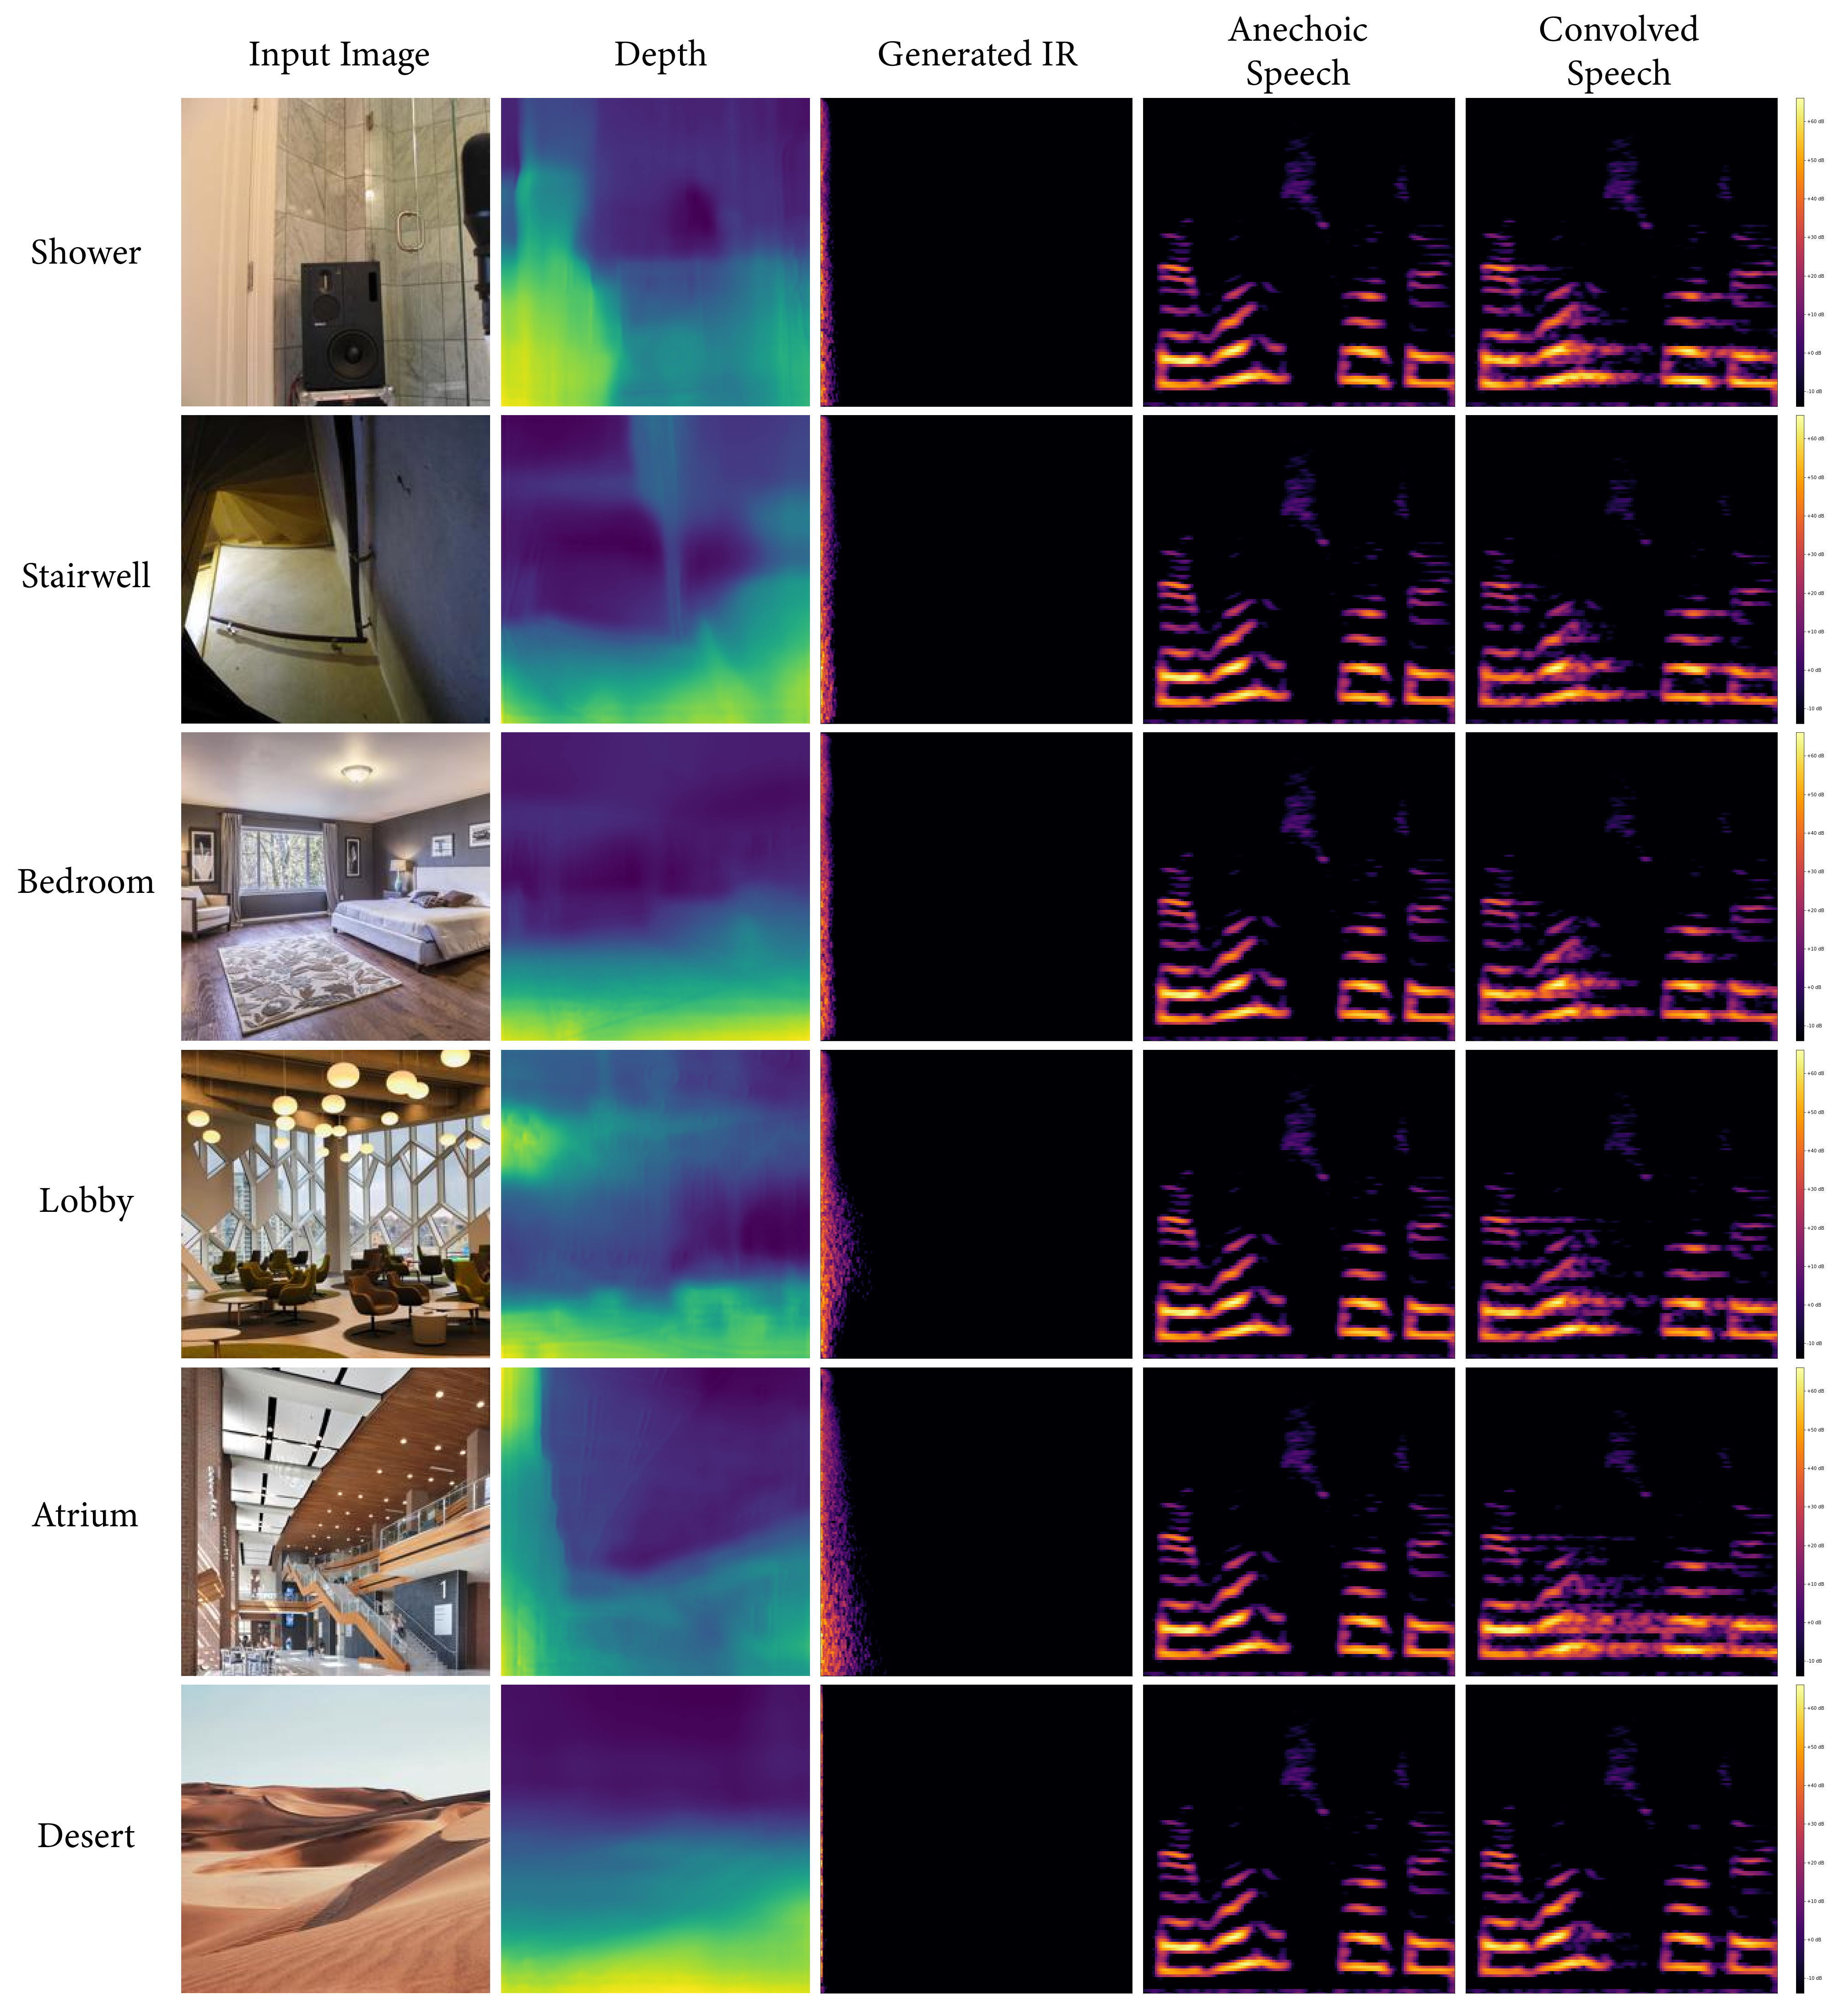
\includegraphics[width=0.9\textwidth]{p_everyday.png}
    \caption{Common and identifiable scenes. Input images and the resulting IRs are shown and convolved with an anechoic speech signal. Input images here reflect spaces that are regularly encountered in everyday life yet may not often be recorded in. These types of scenes are useful for audio post-production as they may be commonly found in movies and television shows. Small and outdoor scenes are observed to have very brief IRs while in comparison, the larger building interior has a much longer output IR as expected.}
    \label{fig:p_everyday}
\end{figure*}

\begin{figure*}[!hb]
    \centering
    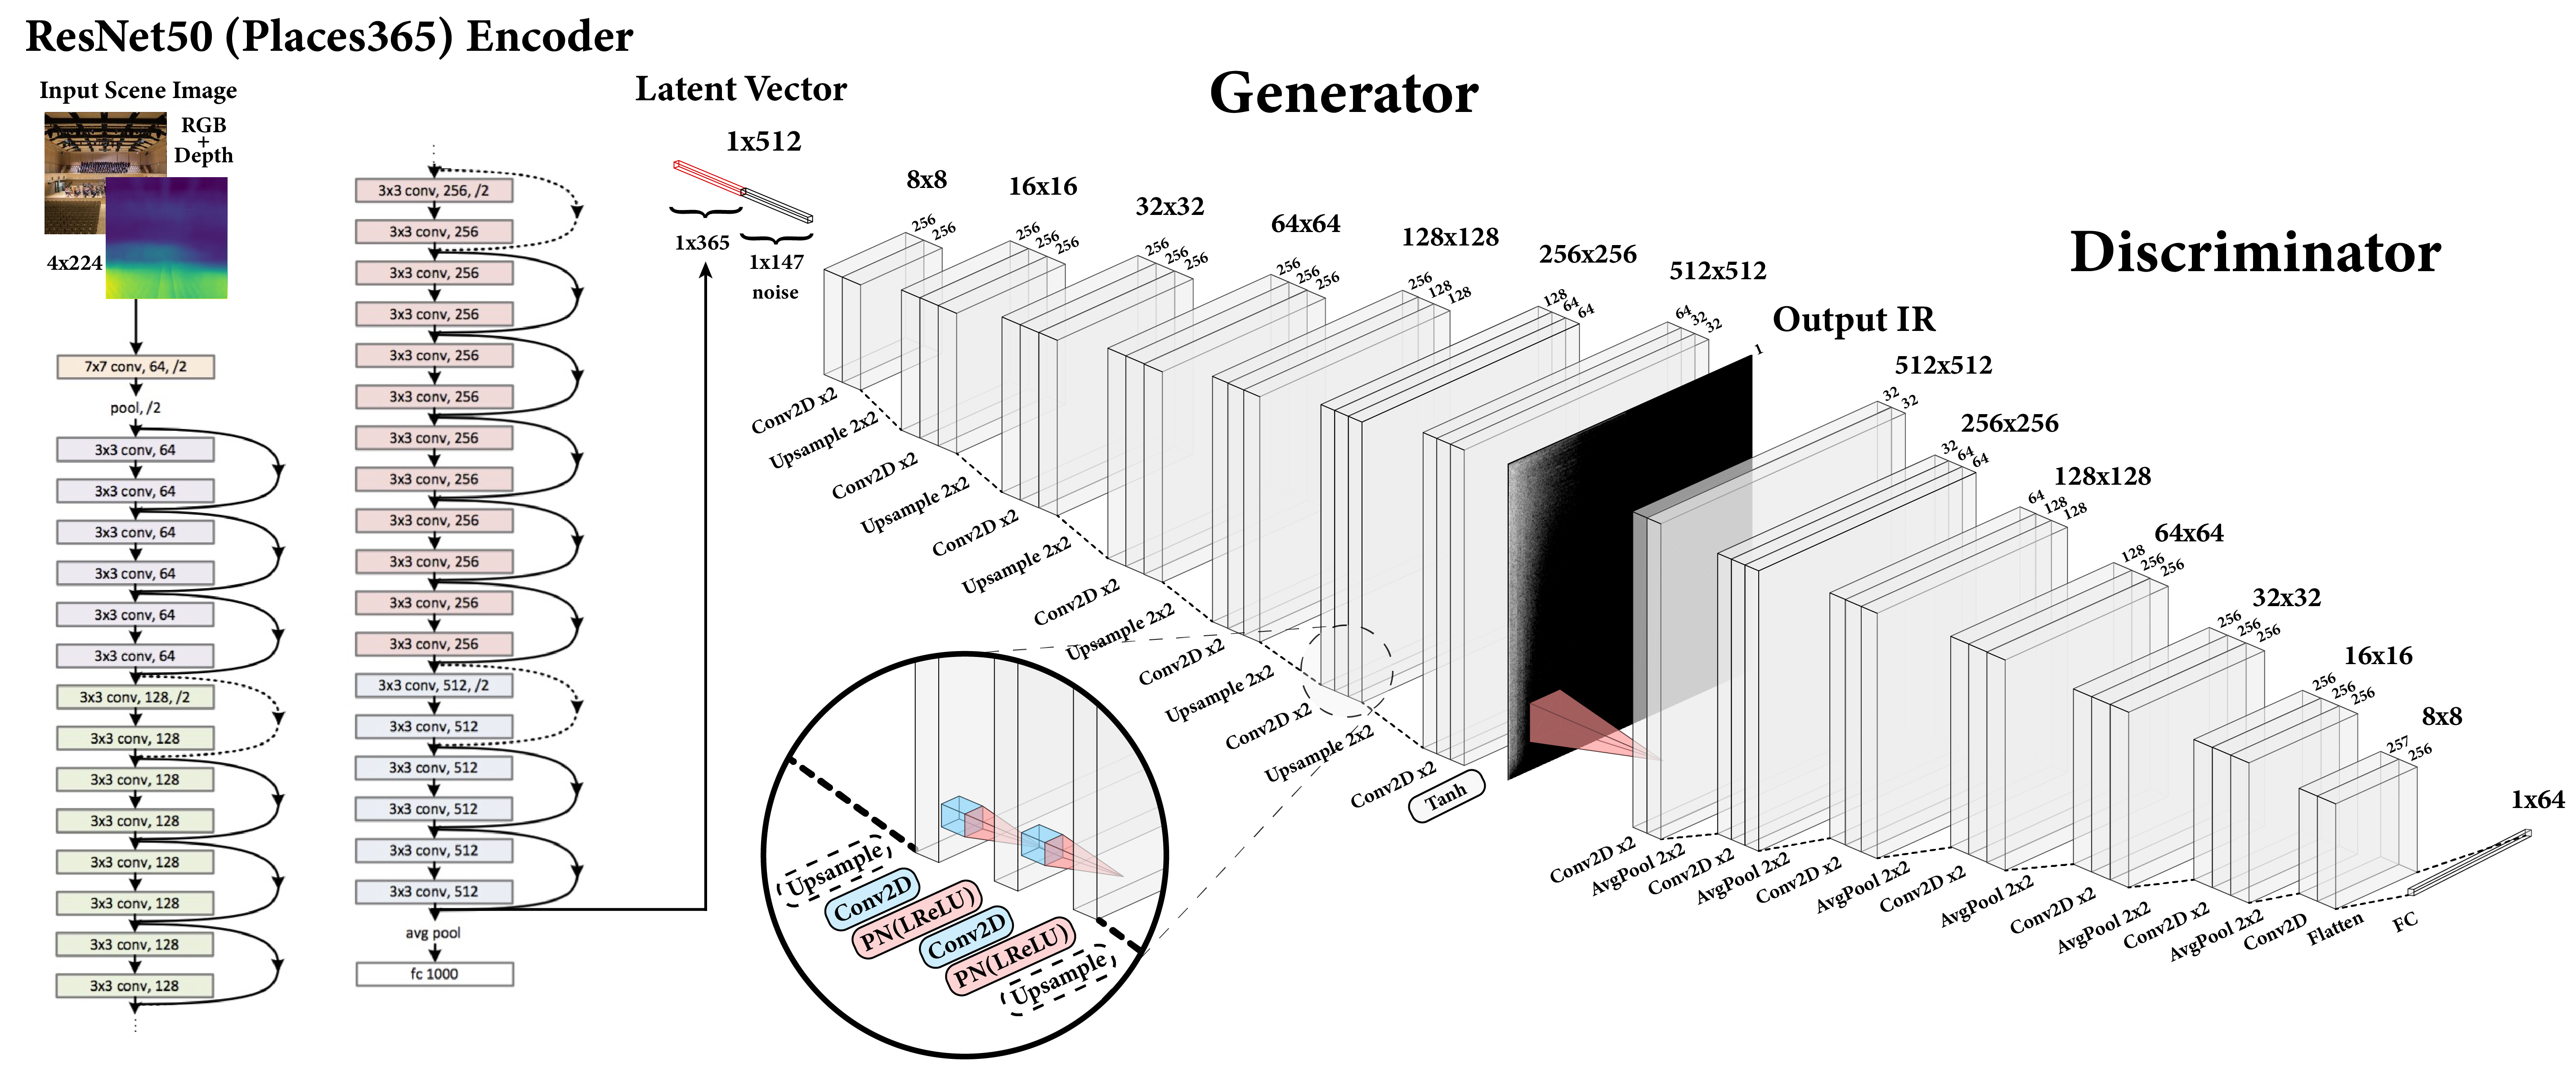
\includegraphics[width=\textwidth]{nn_arch.png}
    \caption{Detailed overview of Image2Reverb model architecture. Left: the ResNet50 encoder pre-trained on Places365 (figure at left adapted from \cite{he2016deep}). Right: the generator and discriminator. The output of the encoder consists of 365 features, to which we concatenate noise to produce a 512d latent vector. The generator and discriminator contain upsampling and downsampling convolutions respectively. A leaky rectified linear unit (LReLU), with $\alpha=0.2$, is used after each convolutional layer in the model in both the discriminator and the generator with the final layer of the generator using a $\tanh$ activation. PN denotes pixelwise normalization, which we use in the generator. The composition of blocks is based on ProGAN \cite{karras2018progressive}. The final step in the discriminator is a fully connected layer with a linear activation (scalar output).}
    \label{fig:nn_arch}
\end{figure*}

\begin{figure*}
    \centering
    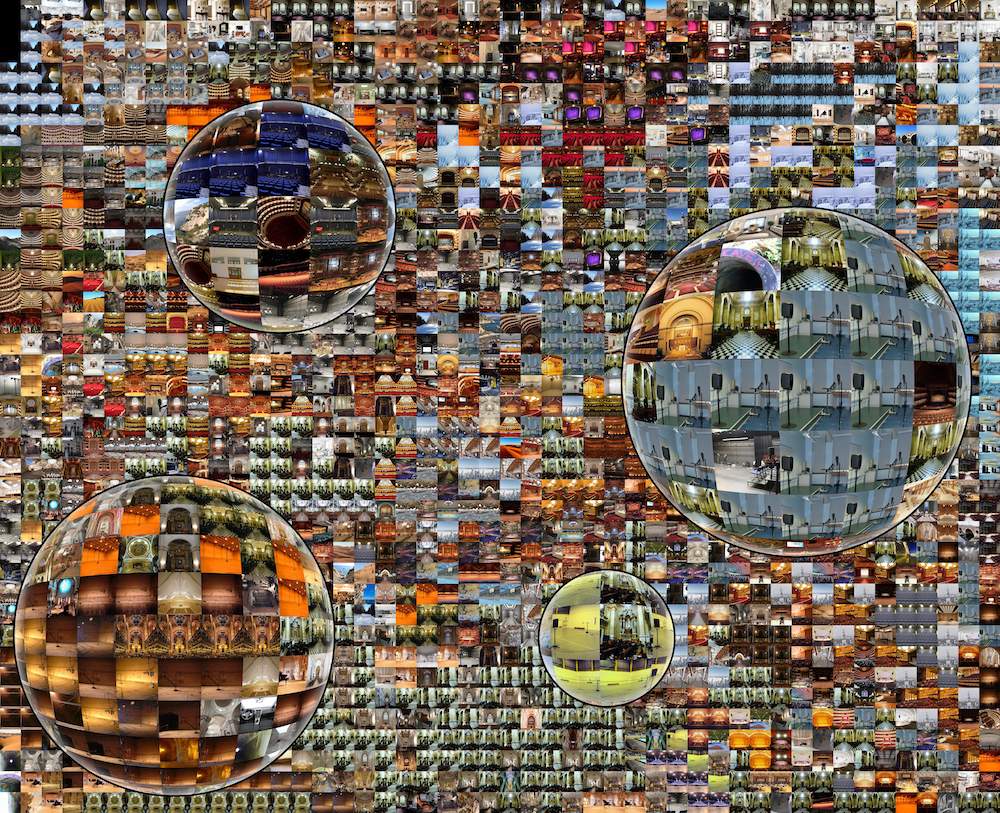
\includegraphics[width=\textwidth]{dataset_tsne2.png}
    \caption{Manifold-based visualization of our test set. We compute multi-band $T_{60}$ estimates for output audio IRs for each image, and then perform nonlinear dimensionality reduction with t-SNE to obtain two-dimensional feature vectors for each example. We produce a grid by solving a linear assignment problem, as is commonly done to visualize large image datasets. Our visualization shows local clusters of same and similar scenes in many cases, but also some variation within scenes. In some outdoor settings, this variation grows considerably large, resulting in increased scattering. In other cases, we observe closeness between different views of the same scene and similar scenes.}
    \label{fig:tsne}
\end{figure*}